\documentclass[twoside]{book}

% Packages required by doxygen
\usepackage{fixltx2e}
\usepackage{calc}
\usepackage{doxygen}
\usepackage[export]{adjustbox} % also loads graphicx
\usepackage{graphicx}
\usepackage[utf8]{inputenc}
\usepackage{makeidx}
\usepackage{multicol}
\usepackage{multirow}
\PassOptionsToPackage{warn}{textcomp}
\usepackage{textcomp}
\usepackage[nointegrals]{wasysym}
\usepackage[table]{xcolor}

% Font selection
\usepackage[T1]{fontenc}
\usepackage[scaled=.90]{helvet}
\usepackage{courier}
\usepackage{amssymb}
\usepackage{sectsty}
\renewcommand{\familydefault}{\sfdefault}
\allsectionsfont{%
  \fontseries{bc}\selectfont%
  \color{darkgray}%
}
\renewcommand{\DoxyLabelFont}{%
  \fontseries{bc}\selectfont%
  \color{darkgray}%
}
\newcommand{\+}{\discretionary{\mbox{\scriptsize$\hookleftarrow$}}{}{}}

% Page & text layout
\usepackage{geometry}
\geometry{%
  a4paper,%
  top=2.5cm,%
  bottom=2.5cm,%
  left=2.5cm,%
  right=2.5cm%
}
\tolerance=750
\hfuzz=15pt
\hbadness=750
\setlength{\emergencystretch}{15pt}
\setlength{\parindent}{0cm}
\setlength{\parskip}{0.2cm}
\makeatletter
\renewcommand{\paragraph}{%
  \@startsection{paragraph}{4}{0ex}{-1.0ex}{1.0ex}{%
    \normalfont\normalsize\bfseries\SS@parafont%
  }%
}
\renewcommand{\subparagraph}{%
  \@startsection{subparagraph}{5}{0ex}{-1.0ex}{1.0ex}{%
    \normalfont\normalsize\bfseries\SS@subparafont%
  }%
}
\makeatother

% Headers & footers
\usepackage{fancyhdr}
\pagestyle{fancyplain}
\fancyhead[LE]{\fancyplain{}{\bfseries\thepage}}
\fancyhead[CE]{\fancyplain{}{}}
\fancyhead[RE]{\fancyplain{}{\bfseries\leftmark}}
\fancyhead[LO]{\fancyplain{}{\bfseries\rightmark}}
\fancyhead[CO]{\fancyplain{}{}}
\fancyhead[RO]{\fancyplain{}{\bfseries\thepage}}
\fancyfoot[LE]{\fancyplain{}{}}
\fancyfoot[CE]{\fancyplain{}{}}
\fancyfoot[RE]{\fancyplain{}{\bfseries\scriptsize Generated on Fri Apr 3 2015 18\+:41\+:37 for Z\+E\+G\+L by Doxygen }}
\fancyfoot[LO]{\fancyplain{}{\bfseries\scriptsize Generated on Fri Apr 3 2015 18\+:41\+:37 for Z\+E\+G\+L by Doxygen }}
\fancyfoot[CO]{\fancyplain{}{}}
\fancyfoot[RO]{\fancyplain{}{}}
\renewcommand{\footrulewidth}{0.4pt}
\renewcommand{\chaptermark}[1]{%
  \markboth{#1}{}%
}
\renewcommand{\sectionmark}[1]{%
  \markright{\thesection\ #1}%
}

% Indices & bibliography
\usepackage{natbib}
\usepackage[titles]{tocloft}
\setcounter{tocdepth}{3}
\setcounter{secnumdepth}{5}
\makeindex

% Hyperlinks (required, but should be loaded last)
\usepackage{ifpdf}
\ifpdf
  \usepackage[pdftex,pagebackref=true]{hyperref}
\else
  \usepackage[ps2pdf,pagebackref=true]{hyperref}
\fi
\hypersetup{%
  colorlinks=true,%
  linkcolor=blue,%
  citecolor=blue,%
  unicode%
}

% Custom commands
\newcommand{\clearemptydoublepage}{%
  \newpage{\pagestyle{empty}\cleardoublepage}%
}


%===== C O N T E N T S =====

\begin{document}

% Titlepage & ToC
\hypersetup{pageanchor=false,
             bookmarks=true,
             bookmarksnumbered=true,
             pdfencoding=unicode
            }
\pagenumbering{roman}
\begin{titlepage}
\vspace*{7cm}
\begin{center}%
{\Large Z\+E\+G\+L }\\
\vspace*{1cm}
{\large Generated by Doxygen 1.8.9.1}\\
\vspace*{0.5cm}
{\small Fri Apr 3 2015 18:41:37}\\
\end{center}
\end{titlepage}
\clearemptydoublepage
\tableofcontents
\clearemptydoublepage
\pagenumbering{arabic}
\hypersetup{pageanchor=true}

%--- Begin generated contents ---
\chapter{Z\+E\+G\+L Index Page}
\label{index}\hypertarget{index}{}\hypertarget{index_LICENSE}{}\section{L\+I\+C\+E\+N\+S\+E}\label{index_LICENSE}
Copyright(c) 2014, Phil Sampson

\href{http://www.zamma.co.uk}{\tt http\+://www.\+zamma.\+co.\+uk}

Licensed under the Apache License, Version 2.\+0 (the \char`\"{}\+License\char`\"{}); you may not use this file except in compliance with the License. You may obtain a copy of the License at

\href{http://www.apache.org/licenses/LICENSE-2.0}{\tt http\+://www.\+apache.\+org/licenses/\+L\+I\+C\+E\+N\+S\+E-\/2.\+0}

Unless required by applicable law or agreed to in writing, software distributed under the License is distributed on an \char`\"{}\+A\+S I\+S\char`\"{} B\+A\+S\+I\+S, W\+I\+T\+H\+O\+U\+T W\+A\+R\+R\+A\+N\+T\+I\+E\+S O\+R C\+O\+N\+D\+I\+T\+I\+O\+N\+S O\+F A\+N\+Y K\+I\+N\+D, either express or implied. See the License for the specific language governing permissions and limitations under the License.\hypertarget{index_intro_sec}{}\section{Introduction}\label{index_intro_sec}
This game engine has been developed in C++ using the following libraries / extensions


\begin{DoxyItemize}
\item \href{https://www.libsdl.org/index.php}{\tt S\+D\+L2}
\item \href{https://www.opengl.org/}{\tt Open\+G\+L 3.\+x}
\item \href{http://glm.g-truc.net/0.9.6/index.html}{\tt G\+L\+M}
\item \href{http://glew.sourceforge.net/}{\tt G\+L\+E\+W}
\item \href{https://github.com/nothings/stb}{\tt stb\+\_\+image -\/ From the stb project}
\item \href{https://github.com/leethomason/tinyxml2}{\tt tinyxml2}
\item \href{https://github.com/Zammalad/fontstash}{\tt Font\+Stash -\/ Forked and modified for my use}
\end{DoxyItemize}

All library and dll files are packaged with the source so there is no need to download them. This helps ensure that the compatibility is maintained if new versions are released.

The {\ttfamily Game} class is designed to be used as a base class and inherited from to create each new game. Once implemented, your main.\+cpp file should look like this (where {\ttfamily My\+Game} is your inherited game class)

An example is included with the source.


\begin{DoxyCode}
\textcolor{preprocessor}{#include "platform.h"}
\textcolor{preprocessor}{#include "core.h"}
\textcolor{preprocessor}{#include "mygame.h"}
\textcolor{preprocessor}{#include "logger.h"}
\textcolor{preprocessor}{#include "system.h"}
\textcolor{preprocessor}{#include "util.h"}
\textcolor{preprocessor}{#include "window.h"}

\textcolor{keyword}{using namespace }\hyperlink{namespace_z_e_g_l}{ZEGL};

\textcolor{keywordtype}{int} main(\textcolor{keywordtype}{int} argc, \textcolor{keywordtype}{char} *argv[])
\{
  \textcolor{comment}{// Initialize the logger class and pass a filename}
  LOG\_INIT(\textcolor{stringliteral}{"ZEGL"});

  \textcolor{comment}{// Perform system initialization}
  \textcolor{keywordflow}{if} (\hyperlink{namespace_z_e_g_l_a2532f9e624be5cdf7898893a8ed3beb5}{ZEGL::Init}())
  \{
    \textcolor{comment}{// Create a window with width 800, height 600 and a title}
    \hyperlink{class_z_e_g_l_1_1_window}{Window} window(800, 600, \textcolor{stringliteral}{"ZEGL"});
    MyGame game;

    \textcolor{comment}{// Create the core system passing in the desired target fps}
    / and pointers to the window and game just created
    \hyperlink{class_z_e_g_l_1_1_core}{Core} engine(60, &window, &game);
    \textcolor{comment}{// Enter the game loop}
    engine.Start();

    \textcolor{comment}{// System cleanup}
    ZEGL::Quit();
  \}

  \textcolor{comment}{// Finish logging}
  LOG\_CLOSE();

  \textcolor{keywordflow}{return} 0;
\}
\end{DoxyCode}
 
\chapter{Namespace Index}
\section{Namespace List}
Here is a list of all documented namespaces with brief descriptions\+:\begin{DoxyCompactList}
\item\contentsline{section}{\hyperlink{namespace_logger}{Logger} }{\pageref{namespace_logger}}{}
\item\contentsline{section}{\hyperlink{namespace_random}{Random} }{\pageref{namespace_random}}{}
\item\contentsline{section}{\hyperlink{namespace_time}{Time} }{\pageref{namespace_time}}{}
\item\contentsline{section}{\hyperlink{namespace_z_e_g_l}{Z\+E\+G\+L} }{\pageref{namespace_z_e_g_l}}{}
\end{DoxyCompactList}

\chapter{Hierarchical Index}
\section{Class Hierarchy}
This inheritance list is sorted roughly, but not completely, alphabetically\+:\begin{DoxyCompactList}
\item \contentsline{section}{Z\+E\+G\+L\+:\+:Core}{\pageref{class_z_e_g_l_1_1_core}}{}
\item \contentsline{section}{Z\+E\+G\+L\+:\+:Entity}{\pageref{class_z_e_g_l_1_1_entity}}{}
\begin{DoxyCompactList}
\item \contentsline{section}{Z\+E\+G\+L\+:\+:Render\+Entity}{\pageref{class_z_e_g_l_1_1_render_entity}}{}
\begin{DoxyCompactList}
\item \contentsline{section}{Z\+E\+G\+L\+:\+:Tile}{\pageref{class_z_e_g_l_1_1_tile}}{}
\end{DoxyCompactList}
\end{DoxyCompactList}
\item \contentsline{section}{Z\+E\+G\+L\+:\+:Entity\+Data}{\pageref{struct_z_e_g_l_1_1_entity_data}}{}
\item \contentsline{section}{Z\+E\+G\+L\+:\+:Game}{\pageref{class_z_e_g_l_1_1_game}}{}
\item \contentsline{section}{Z\+E\+G\+L\+:\+:Input}{\pageref{class_z_e_g_l_1_1_input}}{}
\item \contentsline{section}{Util\+:\+:My\+Singleton$<$ T $>$}{\pageref{class_util_1_1_my_singleton}}{}
\item \contentsline{section}{Z\+E\+G\+L\+:\+:Reference\+Counter}{\pageref{class_z_e_g_l_1_1_reference_counter}}{}
\begin{DoxyCompactList}
\item \contentsline{section}{Z\+E\+G\+L\+:\+:Shader\+Data}{\pageref{class_z_e_g_l_1_1_shader_data}}{}
\item \contentsline{section}{Z\+E\+G\+L\+:\+:Texture\+Atlas\+Data}{\pageref{class_z_e_g_l_1_1_texture_atlas_data}}{}
\item \contentsline{section}{Z\+E\+G\+L\+:\+:Texture\+Data}{\pageref{class_z_e_g_l_1_1_texture_data}}{}
\end{DoxyCompactList}
\item \contentsline{section}{Z\+E\+G\+L\+:\+:Shader}{\pageref{class_z_e_g_l_1_1_shader}}{}
\item \contentsline{section}{Z\+E\+G\+L\+:\+:Texture}{\pageref{class_z_e_g_l_1_1_texture}}{}
\item \contentsline{section}{Z\+E\+G\+L\+:\+:Texture\+Atlas}{\pageref{class_z_e_g_l_1_1_texture_atlas}}{}
\item \contentsline{section}{Z\+E\+G\+L\+:\+:Texture\+Region}{\pageref{struct_z_e_g_l_1_1_texture_region}}{}
\item \contentsline{section}{Z\+E\+G\+L\+:\+:Tile\+Definition}{\pageref{struct_z_e_g_l_1_1_tile_definition}}{}
\item \contentsline{section}{Z\+E\+G\+L\+:\+:Tile\+Map}{\pageref{class_z_e_g_l_1_1_tile_map}}{}
\item \contentsline{section}{Z\+E\+G\+L\+:\+:Timer}{\pageref{class_z_e_g_l_1_1_timer}}{}
\item \contentsline{section}{Z\+E\+G\+L\+:\+:Window}{\pageref{class_z_e_g_l_1_1_window}}{}
\end{DoxyCompactList}

\chapter{Class Index}
\section{Class List}
Here are the classes, structs, unions and interfaces with brief descriptions\+:\begin{DoxyCompactList}
\item\contentsline{section}{\hyperlink{class_z_e_g_l_1_1_camera}{Z\+E\+G\+L\+::\+Camera} }{\pageref{class_z_e_g_l_1_1_camera}}{}
\item\contentsline{section}{\hyperlink{class_z_e_g_l_1_1_core}{Z\+E\+G\+L\+::\+Core} }{\pageref{class_z_e_g_l_1_1_core}}{}
\item\contentsline{section}{\hyperlink{class_z_e_g_l_1_1_entity}{Z\+E\+G\+L\+::\+Entity} }{\pageref{class_z_e_g_l_1_1_entity}}{}
\item\contentsline{section}{\hyperlink{struct_z_e_g_l_1_1_entity_data}{Z\+E\+G\+L\+::\+Entity\+Data} }{\pageref{struct_z_e_g_l_1_1_entity_data}}{}
\item\contentsline{section}{\hyperlink{class_z_e_g_l_1_1_game}{Z\+E\+G\+L\+::\+Game} }{\pageref{class_z_e_g_l_1_1_game}}{}
\item\contentsline{section}{\hyperlink{class_z_e_g_l_1_1_input}{Z\+E\+G\+L\+::\+Input} }{\pageref{class_z_e_g_l_1_1_input}}{}
\item\contentsline{section}{\hyperlink{class_z_e_g_l_1_1_light}{Z\+E\+G\+L\+::\+Light} }{\pageref{class_z_e_g_l_1_1_light}}{}
\item\contentsline{section}{\hyperlink{class_util_1_1_my_singleton}{Util\+::\+My\+Singleton$<$ T $>$} }{\pageref{class_util_1_1_my_singleton}}{}
\item\contentsline{section}{\hyperlink{class_z_e_g_l_1_1_reference_counter}{Z\+E\+G\+L\+::\+Reference\+Counter} }{\pageref{class_z_e_g_l_1_1_reference_counter}}{}
\item\contentsline{section}{\hyperlink{class_z_e_g_l_1_1_render_entity}{Z\+E\+G\+L\+::\+Render\+Entity} }{\pageref{class_z_e_g_l_1_1_render_entity}}{}
\item\contentsline{section}{\hyperlink{class_z_e_g_l_1_1_shader}{Z\+E\+G\+L\+::\+Shader} }{\pageref{class_z_e_g_l_1_1_shader}}{}
\item\contentsline{section}{\hyperlink{class_z_e_g_l_1_1_shader_data}{Z\+E\+G\+L\+::\+Shader\+Data} }{\pageref{class_z_e_g_l_1_1_shader_data}}{}
\item\contentsline{section}{\hyperlink{class_z_e_g_l_1_1_texture}{Z\+E\+G\+L\+::\+Texture} }{\pageref{class_z_e_g_l_1_1_texture}}{}
\item\contentsline{section}{\hyperlink{class_z_e_g_l_1_1_texture_atlas}{Z\+E\+G\+L\+::\+Texture\+Atlas} }{\pageref{class_z_e_g_l_1_1_texture_atlas}}{}
\item\contentsline{section}{\hyperlink{class_z_e_g_l_1_1_texture_atlas_data}{Z\+E\+G\+L\+::\+Texture\+Atlas\+Data} }{\pageref{class_z_e_g_l_1_1_texture_atlas_data}}{}
\item\contentsline{section}{\hyperlink{class_z_e_g_l_1_1_texture_data}{Z\+E\+G\+L\+::\+Texture\+Data} }{\pageref{class_z_e_g_l_1_1_texture_data}}{}
\item\contentsline{section}{\hyperlink{struct_z_e_g_l_1_1_texture_region}{Z\+E\+G\+L\+::\+Texture\+Region} }{\pageref{struct_z_e_g_l_1_1_texture_region}}{}
\item\contentsline{section}{\hyperlink{class_z_e_g_l_1_1_tile}{Z\+E\+G\+L\+::\+Tile} }{\pageref{class_z_e_g_l_1_1_tile}}{}
\item\contentsline{section}{\hyperlink{struct_z_e_g_l_1_1_tile_definition}{Z\+E\+G\+L\+::\+Tile\+Definition} }{\pageref{struct_z_e_g_l_1_1_tile_definition}}{}
\item\contentsline{section}{\hyperlink{class_z_e_g_l_1_1_tile_map}{Z\+E\+G\+L\+::\+Tile\+Map} }{\pageref{class_z_e_g_l_1_1_tile_map}}{}
\item\contentsline{section}{\hyperlink{class_z_e_g_l_1_1_timer}{Z\+E\+G\+L\+::\+Timer} }{\pageref{class_z_e_g_l_1_1_timer}}{}
\item\contentsline{section}{\hyperlink{class_z_e_g_l_1_1_window}{Z\+E\+G\+L\+::\+Window} }{\pageref{class_z_e_g_l_1_1_window}}{}
\end{DoxyCompactList}

\chapter{Namespace Documentation}
\hypertarget{namespace_logger}{}\section{Logger Namespace Reference}
\label{namespace_logger}\index{Logger@{Logger}}
\subsection*{Functions}
\begin{DoxyCompactItemize}
\item 
\hypertarget{namespace_logger_a0a67d9cca642837b53f12b97e8d8ed75}{}void {\bfseries Init} (const std\+::string \&fname)\label{namespace_logger_a0a67d9cca642837b53f12b97e8d8ed75}

\item 
\hypertarget{namespace_logger_ae390b2c3819cf54bf112f0a2f9a9b116}{}void {\bfseries New\+Line} ()\label{namespace_logger_ae390b2c3819cf54bf112f0a2f9a9b116}

\item 
\hypertarget{namespace_logger_aee61421bdb0c854d2f203f41c396ef59}{}void {\bfseries Log\+Info} (const std\+::string \&msg)\label{namespace_logger_aee61421bdb0c854d2f203f41c396ef59}

\item 
\hypertarget{namespace_logger_a4fd5b8d79ca7daff30a32e42cda36511}{}void {\bfseries Log\+Warning} (const std\+::string \&msg)\label{namespace_logger_a4fd5b8d79ca7daff30a32e42cda36511}

\item 
\hypertarget{namespace_logger_adf5325af43de366d89b9dcc882b9c8c6}{}void {\bfseries Log\+Error} (const std\+::string \&msg)\label{namespace_logger_adf5325af43de366d89b9dcc882b9c8c6}

\item 
\hypertarget{namespace_logger_ab13114d60ca5f1f69f2ba0f2f1a5bd19}{}void {\bfseries Close} ()\label{namespace_logger_ab13114d60ca5f1f69f2ba0f2f1a5bd19}

\end{DoxyCompactItemize}


\subsection{Detailed Description}
Copyright(c) 2014, Phil Sampson (\href{http://www.zamma.co.uk}{\tt http\+://www.\+zamma.\+co.\+uk})

Licensed under the Apache License, Version 2.\+0 (the \char`\"{}\+License\char`\"{}); you may not use this file except in compliance with the License. You may obtain a copy of the License at

\href{http://www.apache.org/licenses/LICENSE-2.0}{\tt http\+://www.\+apache.\+org/licenses/\+L\+I\+C\+E\+N\+S\+E-\/2.\+0}

Unless required by applicable law or agreed to in writing, software distributed under the License is distributed on an \char`\"{}\+A\+S I\+S\char`\"{} B\+A\+S\+I\+S, W\+I\+T\+H\+O\+U\+T W\+A\+R\+R\+A\+N\+T\+I\+E\+S O\+R C\+O\+N\+D\+I\+T\+I\+O\+N\+S O\+F A\+N\+Y K\+I\+N\+D, either express or implied. See the License for the specific language governing permissions and limitations under the License. 
\hypertarget{namespace_random}{}\section{Random Namespace Reference}
\label{namespace_random}\index{Random@{Random}}
\subsection*{Functions}
\begin{DoxyCompactItemize}
\item 
\hypertarget{namespace_random_a9feade8fc8026ed3e7aad3b1cdd9b55a}{}void {\bfseries Init} ()\label{namespace_random_a9feade8fc8026ed3e7aad3b1cdd9b55a}

\item 
\hypertarget{namespace_random_a1df1df554acc51763182dc0feffabb45}{}int {\bfseries Rand\+Int} (int max)\label{namespace_random_a1df1df554acc51763182dc0feffabb45}

\item 
\hypertarget{namespace_random_af95f32ab928b256643961ed85ada5d9b}{}int {\bfseries Rand\+Int} (int min, int max)\label{namespace_random_af95f32ab928b256643961ed85ada5d9b}

\item 
\hypertarget{namespace_random_ae424eea89fb07462a98df20e6989942e}{}float {\bfseries Rand\+Float} (float max)\label{namespace_random_ae424eea89fb07462a98df20e6989942e}

\item 
\hypertarget{namespace_random_ac2d5dc2c33542e40dffc0750c5d06e38}{}float {\bfseries Rand\+Float} (float min, float max)\label{namespace_random_ac2d5dc2c33542e40dffc0750c5d06e38}

\item 
\hypertarget{namespace_random_afb12a70247db5c12a6f79134d2d8abc3}{}bool {\bfseries Rand\+Bool} ()\label{namespace_random_afb12a70247db5c12a6f79134d2d8abc3}

\end{DoxyCompactItemize}


\subsection{Detailed Description}
Copyright(c) 2014, Phil Sampson (\href{http://www.zamma.co.uk}{\tt http\+://www.\+zamma.\+co.\+uk})

Licensed under the Apache License, Version 2.\+0 (the \char`\"{}\+License\char`\"{}); you may not use this file except in compliance with the License. You may obtain a copy of the License at

\href{http://www.apache.org/licenses/LICENSE-2.0}{\tt http\+://www.\+apache.\+org/licenses/\+L\+I\+C\+E\+N\+S\+E-\/2.\+0}

Unless required by applicable law or agreed to in writing, software distributed under the License is distributed on an \char`\"{}\+A\+S I\+S\char`\"{} B\+A\+S\+I\+S, W\+I\+T\+H\+O\+U\+T W\+A\+R\+R\+A\+N\+T\+I\+E\+S O\+R C\+O\+N\+D\+I\+T\+I\+O\+N\+S O\+F A\+N\+Y K\+I\+N\+D, either express or implied. See the License for the specific language governing permissions and limitations under the License. 
\hypertarget{namespace_time}{}\section{Time Namespace Reference}
\label{namespace_time}\index{Time@{Time}}
\subsection*{Functions}
\begin{DoxyCompactItemize}
\item 
\hypertarget{namespace_time_aa5dcef5b8d122df3f323afd164dd67f7}{}double {\bfseries Get\+Time} ()\label{namespace_time_aa5dcef5b8d122df3f323afd164dd67f7}

\end{DoxyCompactItemize}


\subsection{Detailed Description}
Copyright(c) 2014, Phil Sampson (\href{http://www.zamma.co.uk}{\tt http\+://www.\+zamma.\+co.\+uk})

Licensed under the Apache License, Version 2.\+0 (the \char`\"{}\+License\char`\"{}); you may not use this file except in compliance with the License. You may obtain a copy of the License at

\href{http://www.apache.org/licenses/LICENSE-2.0}{\tt http\+://www.\+apache.\+org/licenses/\+L\+I\+C\+E\+N\+S\+E-\/2.\+0}

Unless required by applicable law or agreed to in writing, software distributed under the License is distributed on an \char`\"{}\+A\+S I\+S\char`\"{} B\+A\+S\+I\+S, W\+I\+T\+H\+O\+U\+T W\+A\+R\+R\+A\+N\+T\+I\+E\+S O\+R C\+O\+N\+D\+I\+T\+I\+O\+N\+S O\+F A\+N\+Y K\+I\+N\+D, either express or implied. See the License for the specific language governing permissions and limitations under the License. 
\hypertarget{namespace_z_e_g_l}{}\section{Z\+E\+G\+L Namespace Reference}
\label{namespace_z_e_g_l}\index{Z\+E\+G\+L@{Z\+E\+G\+L}}
\subsection*{Classes}
\begin{DoxyCompactItemize}
\item 
class \hyperlink{class_z_e_g_l_1_1_camera}{Camera}
\item 
class \hyperlink{class_z_e_g_l_1_1_core}{Core}
\item 
class \hyperlink{class_z_e_g_l_1_1_entity}{Entity}
\item 
struct \hyperlink{struct_z_e_g_l_1_1_entity_data}{Entity\+Data}
\item 
class \hyperlink{class_z_e_g_l_1_1_game}{Game}
\item 
class \hyperlink{class_z_e_g_l_1_1_input}{Input}
\item 
class \hyperlink{class_z_e_g_l_1_1_light}{Light}
\item 
class \hyperlink{class_z_e_g_l_1_1_reference_counter}{Reference\+Counter}
\item 
class \hyperlink{class_z_e_g_l_1_1_render_entity}{Render\+Entity}
\item 
class \hyperlink{class_z_e_g_l_1_1_shader}{Shader}
\item 
class \hyperlink{class_z_e_g_l_1_1_shader_data}{Shader\+Data}
\item 
class \hyperlink{class_z_e_g_l_1_1_texture}{Texture}
\item 
class \hyperlink{class_z_e_g_l_1_1_texture_atlas}{Texture\+Atlas}
\item 
class \hyperlink{class_z_e_g_l_1_1_texture_atlas_data}{Texture\+Atlas\+Data}
\item 
class \hyperlink{class_z_e_g_l_1_1_texture_data}{Texture\+Data}
\item 
struct \hyperlink{struct_z_e_g_l_1_1_texture_region}{Texture\+Region}
\item 
class \hyperlink{class_z_e_g_l_1_1_tile}{Tile}
\item 
struct \hyperlink{struct_z_e_g_l_1_1_tile_definition}{Tile\+Definition}
\item 
class \hyperlink{class_z_e_g_l_1_1_tile_map}{Tile\+Map}
\item 
class \hyperlink{class_z_e_g_l_1_1_timer}{Timer}
\item 
class \hyperlink{class_z_e_g_l_1_1_window}{Window}
\end{DoxyCompactItemize}
\subsection*{Functions}
\begin{DoxyCompactItemize}
\item 
bool \hyperlink{namespace_z_e_g_l_a2532f9e624be5cdf7898893a8ed3beb5}{Init} ()
\item 
\hypertarget{namespace_z_e_g_l_ac2c7a1737692877ad76697a69cf537e5}{}void {\bfseries Quit} ()\label{namespace_z_e_g_l_ac2c7a1737692877ad76697a69cf537e5}

\item 
\hypertarget{namespace_z_e_g_l_a0a2ded953044c4b444be741c7e2df2a2}{}void {\bfseries Log\+S\+D\+L\+Info} ()\label{namespace_z_e_g_l_a0a2ded953044c4b444be741c7e2df2a2}

\item 
\hypertarget{namespace_z_e_g_l_a38968dd1324a1df01bb2eeefddb94396}{}void {\bfseries Log\+System\+Info} ()\label{namespace_z_e_g_l_a38968dd1324a1df01bb2eeefddb94396}

\item 
\hypertarget{namespace_z_e_g_l_a7cc637f694bcda7c8bca91e4b8befa86}{}void {\bfseries Log\+Sub\+System\+Info} (S\+D\+L\+\_\+\+Window $\ast$window)\label{namespace_z_e_g_l_a7cc637f694bcda7c8bca91e4b8befa86}

\item 
\hypertarget{namespace_z_e_g_l_a03256a2698fec5ffb6985205c4c9a32e}{}void {\bfseries Log\+O\+S\+Info} ()\label{namespace_z_e_g_l_a03256a2698fec5ffb6985205c4c9a32e}

\item 
\hypertarget{namespace_z_e_g_l_a22a7ea2af1dd5aa5fdcfe38fabcb616f}{}S\+D\+L\+\_\+\+Window $\ast$ {\bfseries Create\+And\+Log\+Window} (const char $\ast$title, int w, int h, Uint32 flags)\label{namespace_z_e_g_l_a22a7ea2af1dd5aa5fdcfe38fabcb616f}

\item 
\hypertarget{namespace_z_e_g_l_a62502e9b394f9879403c71aafdb8e166}{}S\+D\+L\+\_\+\+Window $\ast$ {\bfseries Create\+And\+Log\+Window} (const char $\ast$title, int x, int y, int w, int h, Uint32 flags)\label{namespace_z_e_g_l_a62502e9b394f9879403c71aafdb8e166}

\end{DoxyCompactItemize}
\subsection*{Variables}
\begin{DoxyCompactItemize}
\item 
\hypertarget{namespace_z_e_g_l_a602be510f970fe1ad0f68867132e27af}{}const float {\bfseries D\+E\+F\+A\+U\+L\+T\+\_\+\+T\+I\+L\+E\+\_\+\+S\+I\+Z\+E} = 512.\+0f\label{namespace_z_e_g_l_a602be510f970fe1ad0f68867132e27af}

\end{DoxyCompactItemize}


\subsection{Detailed Description}
Copyright(c) 2014, Phil Sampson (\href{http://www.zamma.co.uk}{\tt http\+://www.\+zamma.\+co.\+uk})

Licensed under the Apache License, Version 2.\+0 (the \char`\"{}\+License\char`\"{}); you may not use this file except in compliance with the License. You may obtain a copy of the License at

\href{http://www.apache.org/licenses/LICENSE-2.0}{\tt http\+://www.\+apache.\+org/licenses/\+L\+I\+C\+E\+N\+S\+E-\/2.\+0}

Unless required by applicable law or agreed to in writing, software distributed under the License is distributed on an \char`\"{}\+A\+S I\+S\char`\"{} B\+A\+S\+I\+S, W\+I\+T\+H\+O\+U\+T W\+A\+R\+R\+A\+N\+T\+I\+E\+S O\+R C\+O\+N\+D\+I\+T\+I\+O\+N\+S O\+F A\+N\+Y K\+I\+N\+D, either express or implied. See the License for the specific language governing permissions and limitations under the License. 

\subsection{Function Documentation}
\hypertarget{namespace_z_e_g_l_a2532f9e624be5cdf7898893a8ed3beb5}{}\index{Z\+E\+G\+L@{Z\+E\+G\+L}!Init@{Init}}
\index{Init@{Init}!Z\+E\+G\+L@{Z\+E\+G\+L}}
\subsubsection[{Init}]{\setlength{\rightskip}{0pt plus 5cm}bool Z\+E\+G\+L\+::\+Init (
\begin{DoxyParamCaption}
{}
\end{DoxyParamCaption}
)}\label{namespace_z_e_g_l_a2532f9e624be5cdf7898893a8ed3beb5}
Copyright(c) 2014, Phil Sampson (\href{http://www.zamma.co.uk}{\tt http\+://www.\+zamma.\+co.\+uk})

Licensed under the Apache License, Version 2.\+0 (the \char`\"{}\+License\char`\"{}); you may not use this file except in compliance with the License. You may obtain a copy of the License at

\href{http://www.apache.org/licenses/LICENSE-2.0}{\tt http\+://www.\+apache.\+org/licenses/\+L\+I\+C\+E\+N\+S\+E-\/2.\+0}

Unless required by applicable law or agreed to in writing, software distributed under the License is distributed on an \char`\"{}\+A\+S I\+S\char`\"{} B\+A\+S\+I\+S, W\+I\+T\+H\+O\+U\+T W\+A\+R\+R\+A\+N\+T\+I\+E\+S O\+R C\+O\+N\+D\+I\+T\+I\+O\+N\+S O\+F A\+N\+Y K\+I\+N\+D, either express or implied. See the License for the specific language governing permissions and limitations under the License. 
\chapter{Class Documentation}
\hypertarget{class_z_e_g_l_1_1_camera}{}\section{Z\+E\+G\+L\+:\+:Camera Class Reference}
\label{class_z_e_g_l_1_1_camera}\index{Z\+E\+G\+L\+::\+Camera@{Z\+E\+G\+L\+::\+Camera}}


{\ttfamily \#include $<$camera.\+h$>$}

\subsection*{Public Member Functions}
\begin{DoxyCompactItemize}
\item 
\hyperlink{class_z_e_g_l_1_1_camera_afe162528fc9249f540aa772c0d1c22c9}{Camera} (const \hyperlink{class_z_e_g_l_1_1_window}{Window} $\ast$window=nullptr)
\item 
const glm\+::mat4 \& \hyperlink{class_z_e_g_l_1_1_camera_ad39df4bd961d2debd682f87f657f9614}{Get\+Transform} (const \hyperlink{class_z_e_g_l_1_1_window}{Window} $\ast$window)
\item 
glm\+::vec3 \hyperlink{class_z_e_g_l_1_1_camera_a0dbdf23ce58ffee1a5a7fcfe7672f1cc}{Get\+Pos} () const 
\item 
void \hyperlink{class_z_e_g_l_1_1_camera_a3e4d6e95cf1c0357937de4b515f88b6b}{Set\+Pos} (float x, float y, float z=0.\+0f)
\item 
float \hyperlink{class_z_e_g_l_1_1_camera_adda8a25f5ba68c3dba29334659a66652}{Get\+Rot} () const 
\item 
void \hyperlink{class_z_e_g_l_1_1_camera_a1c44b901139b76428955637d7eeb000b}{Set\+Rot} (float rot)
\item 
float \hyperlink{class_z_e_g_l_1_1_camera_ae90bbfb4a99f096269973a524a3697d8}{Get\+Zoom} () const 
\item 
void \hyperlink{class_z_e_g_l_1_1_camera_ac487ced7703cdedce8d7b3041cc580d7}{Set\+Zoom} (float zoom)
\item 
\hypertarget{class_z_e_g_l_1_1_camera_a635568a1202e5f39b71b8270e747daae}{}void $\ast$ {\bfseries operator new} (size\+\_\+t i)\label{class_z_e_g_l_1_1_camera_a635568a1202e5f39b71b8270e747daae}

\item 
\hypertarget{class_z_e_g_l_1_1_camera_ab70a6518d82b2cb86163642c27cd6436}{}void {\bfseries operator delete} (void $\ast$p)\label{class_z_e_g_l_1_1_camera_ab70a6518d82b2cb86163642c27cd6436}

\end{DoxyCompactItemize}


\subsection{Detailed Description}
The camera is used for moving the display around the in game world. It uses position, rotation and zoom to create an orthographic transformation matrix which in turn is used for rendering. 

\subsection{Constructor \& Destructor Documentation}
\hypertarget{class_z_e_g_l_1_1_camera_afe162528fc9249f540aa772c0d1c22c9}{}\index{Z\+E\+G\+L\+::\+Camera@{Z\+E\+G\+L\+::\+Camera}!Camera@{Camera}}
\index{Camera@{Camera}!Z\+E\+G\+L\+::\+Camera@{Z\+E\+G\+L\+::\+Camera}}
\subsubsection[{Camera}]{\setlength{\rightskip}{0pt plus 5cm}Camera\+::\+Camera (
\begin{DoxyParamCaption}
\item[{const {\bf Window} $\ast$}]{window = {\ttfamily nullptr}}
\end{DoxyParamCaption}
)}\label{class_z_e_g_l_1_1_camera_afe162528fc9249f540aa772c0d1c22c9}
Constructor.

The constructor uses the \hyperlink{class_z_e_g_l_1_1_window}{Window} which is passed in to calculate a transformation matrix.


\begin{DoxyParams}[1]{Parameters}
\mbox{\tt in}  & {\em window} & Pointer to a \hyperlink{class_z_e_g_l_1_1_window}{Window} (defaults to nullptr)\\
\hline
\end{DoxyParams}
\begin{DoxyWarning}{Warning}
If no \hyperlink{class_z_e_g_l_1_1_window}{Window} is passed a default orthographic projection is used. This is to prevent a crash but should not be used for general purpose i.\+e. make sure you pass a \hyperlink{class_z_e_g_l_1_1_window}{Window} in order to get correct rendering
\end{DoxyWarning}
\begin{DoxySeeAlso}{See also}
\mbox{[}\hyperlink{class_z_e_g_l_1_1_window}{Window}\mbox{]} 
\end{DoxySeeAlso}


\subsection{Member Function Documentation}
\hypertarget{class_z_e_g_l_1_1_camera_a0dbdf23ce58ffee1a5a7fcfe7672f1cc}{}\index{Z\+E\+G\+L\+::\+Camera@{Z\+E\+G\+L\+::\+Camera}!Get\+Pos@{Get\+Pos}}
\index{Get\+Pos@{Get\+Pos}!Z\+E\+G\+L\+::\+Camera@{Z\+E\+G\+L\+::\+Camera}}
\subsubsection[{Get\+Pos}]{\setlength{\rightskip}{0pt plus 5cm}glm\+::vec3 Z\+E\+G\+L\+::\+Camera\+::\+Get\+Pos (
\begin{DoxyParamCaption}
{}
\end{DoxyParamCaption}
) const\hspace{0.3cm}{\ttfamily [inline]}}\label{class_z_e_g_l_1_1_camera_a0dbdf23ce58ffee1a5a7fcfe7672f1cc}
Get the current position of the \hyperlink{class_z_e_g_l_1_1_camera}{Camera}.

\begin{DoxyReturn}{Returns}
glm\+::vec3 representing the \hyperlink{class_z_e_g_l_1_1_camera}{Camera} position 
\end{DoxyReturn}
\hypertarget{class_z_e_g_l_1_1_camera_adda8a25f5ba68c3dba29334659a66652}{}\index{Z\+E\+G\+L\+::\+Camera@{Z\+E\+G\+L\+::\+Camera}!Get\+Rot@{Get\+Rot}}
\index{Get\+Rot@{Get\+Rot}!Z\+E\+G\+L\+::\+Camera@{Z\+E\+G\+L\+::\+Camera}}
\subsubsection[{Get\+Rot}]{\setlength{\rightskip}{0pt plus 5cm}float Z\+E\+G\+L\+::\+Camera\+::\+Get\+Rot (
\begin{DoxyParamCaption}
{}
\end{DoxyParamCaption}
) const\hspace{0.3cm}{\ttfamily [inline]}}\label{class_z_e_g_l_1_1_camera_adda8a25f5ba68c3dba29334659a66652}
Get the current rotation of the \hyperlink{class_z_e_g_l_1_1_camera}{Camera}.

\begin{DoxyReturn}{Returns}
\hyperlink{class_z_e_g_l_1_1_camera}{Camera} rotation in radians 
\end{DoxyReturn}
\hypertarget{class_z_e_g_l_1_1_camera_ad39df4bd961d2debd682f87f657f9614}{}\index{Z\+E\+G\+L\+::\+Camera@{Z\+E\+G\+L\+::\+Camera}!Get\+Transform@{Get\+Transform}}
\index{Get\+Transform@{Get\+Transform}!Z\+E\+G\+L\+::\+Camera@{Z\+E\+G\+L\+::\+Camera}}
\subsubsection[{Get\+Transform}]{\setlength{\rightskip}{0pt plus 5cm}const glm\+::mat4 \& Camera\+::\+Get\+Transform (
\begin{DoxyParamCaption}
\item[{const {\bf Window} $\ast$}]{window}
\end{DoxyParamCaption}
)}\label{class_z_e_g_l_1_1_camera_ad39df4bd961d2debd682f87f657f9614}
Get the current transformation matrix.

If the last position, rotation or zoom value has changed the \hyperlink{class_z_e_g_l_1_1_camera}{Camera} uses the \hyperlink{class_z_e_g_l_1_1_window}{Window} which is passed in to re-\/calculate a transformation matrix.


\begin{DoxyParams}[1]{Parameters}
\mbox{\tt in}  & {\em window} & Pointer to a \hyperlink{class_z_e_g_l_1_1_window}{Window} (defaults to nullptr)\\
\hline
\end{DoxyParams}
\begin{DoxyReturn}{Returns}
glm\+::mat4 Orthographic transformation matrix
\end{DoxyReturn}
\begin{DoxyWarning}{Warning}
If no \hyperlink{class_z_e_g_l_1_1_window}{Window} is passed a default orthographic projection is used. This is to prevent a crash but should not be used for general purpose i.\+e. make sure you pass a \hyperlink{class_z_e_g_l_1_1_window}{Window} in order to get correct rendering.
\end{DoxyWarning}
\begin{DoxySeeAlso}{See also}
\mbox{[}\hyperlink{class_z_e_g_l_1_1_window}{Window}\mbox{]} 
\end{DoxySeeAlso}
\hypertarget{class_z_e_g_l_1_1_camera_ae90bbfb4a99f096269973a524a3697d8}{}\index{Z\+E\+G\+L\+::\+Camera@{Z\+E\+G\+L\+::\+Camera}!Get\+Zoom@{Get\+Zoom}}
\index{Get\+Zoom@{Get\+Zoom}!Z\+E\+G\+L\+::\+Camera@{Z\+E\+G\+L\+::\+Camera}}
\subsubsection[{Get\+Zoom}]{\setlength{\rightskip}{0pt plus 5cm}float Z\+E\+G\+L\+::\+Camera\+::\+Get\+Zoom (
\begin{DoxyParamCaption}
{}
\end{DoxyParamCaption}
) const\hspace{0.3cm}{\ttfamily [inline]}}\label{class_z_e_g_l_1_1_camera_ae90bbfb4a99f096269973a524a3697d8}
Get the current zoom factor of the \hyperlink{class_z_e_g_l_1_1_camera}{Camera}.

\begin{DoxyReturn}{Returns}
Zoom factor for the \hyperlink{class_z_e_g_l_1_1_camera}{Camera} 
\end{DoxyReturn}
\hypertarget{class_z_e_g_l_1_1_camera_a3e4d6e95cf1c0357937de4b515f88b6b}{}\index{Z\+E\+G\+L\+::\+Camera@{Z\+E\+G\+L\+::\+Camera}!Set\+Pos@{Set\+Pos}}
\index{Set\+Pos@{Set\+Pos}!Z\+E\+G\+L\+::\+Camera@{Z\+E\+G\+L\+::\+Camera}}
\subsubsection[{Set\+Pos}]{\setlength{\rightskip}{0pt plus 5cm}void Z\+E\+G\+L\+::\+Camera\+::\+Set\+Pos (
\begin{DoxyParamCaption}
\item[{float}]{x, }
\item[{float}]{y, }
\item[{float}]{z = {\ttfamily 0.0f}}
\end{DoxyParamCaption}
)\hspace{0.3cm}{\ttfamily [inline]}}\label{class_z_e_g_l_1_1_camera_a3e4d6e95cf1c0357937de4b515f88b6b}
Set the position of the \hyperlink{class_z_e_g_l_1_1_camera}{Camera}.


\begin{DoxyParams}[1]{Parameters}
\mbox{\tt in}  & {\em x} & New X position component value \\
\hline
\mbox{\tt in}  & {\em y} & New Y position component value \\
\hline
\mbox{\tt in}  & {\em z} & New Z position component value \\
\hline
\end{DoxyParams}
\hypertarget{class_z_e_g_l_1_1_camera_a1c44b901139b76428955637d7eeb000b}{}\index{Z\+E\+G\+L\+::\+Camera@{Z\+E\+G\+L\+::\+Camera}!Set\+Rot@{Set\+Rot}}
\index{Set\+Rot@{Set\+Rot}!Z\+E\+G\+L\+::\+Camera@{Z\+E\+G\+L\+::\+Camera}}
\subsubsection[{Set\+Rot}]{\setlength{\rightskip}{0pt plus 5cm}void Z\+E\+G\+L\+::\+Camera\+::\+Set\+Rot (
\begin{DoxyParamCaption}
\item[{float}]{rot}
\end{DoxyParamCaption}
)\hspace{0.3cm}{\ttfamily [inline]}}\label{class_z_e_g_l_1_1_camera_a1c44b901139b76428955637d7eeb000b}
Set the \hyperlink{class_z_e_g_l_1_1_camera}{Camera} rotation.


\begin{DoxyParams}[1]{Parameters}
\mbox{\tt in}  & {\em rot} & Angle of rotation in radians \\
\hline
\end{DoxyParams}
\hypertarget{class_z_e_g_l_1_1_camera_ac487ced7703cdedce8d7b3041cc580d7}{}\index{Z\+E\+G\+L\+::\+Camera@{Z\+E\+G\+L\+::\+Camera}!Set\+Zoom@{Set\+Zoom}}
\index{Set\+Zoom@{Set\+Zoom}!Z\+E\+G\+L\+::\+Camera@{Z\+E\+G\+L\+::\+Camera}}
\subsubsection[{Set\+Zoom}]{\setlength{\rightskip}{0pt plus 5cm}void Z\+E\+G\+L\+::\+Camera\+::\+Set\+Zoom (
\begin{DoxyParamCaption}
\item[{float}]{zoom}
\end{DoxyParamCaption}
)\hspace{0.3cm}{\ttfamily [inline]}}\label{class_z_e_g_l_1_1_camera_ac487ced7703cdedce8d7b3041cc580d7}
Set the \hyperlink{class_z_e_g_l_1_1_camera}{Camera} zoom factor.


\begin{DoxyParams}[1]{Parameters}
\mbox{\tt in}  & {\em zoom} & Level of zoom factor (scaling) to apply \\
\hline
\end{DoxyParams}


The documentation for this class was generated from the following files\+:\begin{DoxyCompactItemize}
\item 
include/camera.\+h\item 
src/camera.\+cpp\end{DoxyCompactItemize}

\hypertarget{class_z_e_g_l_1_1_core}{}\section{Z\+E\+G\+L\+:\+:Core Class Reference}
\label{class_z_e_g_l_1_1_core}\index{Z\+E\+G\+L\+::\+Core@{Z\+E\+G\+L\+::\+Core}}


{\ttfamily \#include $<$core.\+h$>$}

\subsection*{Public Member Functions}
\begin{DoxyCompactItemize}
\item 
\hyperlink{class_z_e_g_l_1_1_core_a5a8f95feb47b3057726dbe2554dc8ac5}{Core} (double frame\+Rate, \hyperlink{class_z_e_g_l_1_1_window}{Window} $\ast$window, \hyperlink{class_z_e_g_l_1_1_game}{Game} $\ast$game)
\item 
void \hyperlink{class_z_e_g_l_1_1_core_a44f0db8bca5b6fd85f3948250287bdbd}{Start} ()
\item 
void \hyperlink{class_z_e_g_l_1_1_core_acab57c44acf4231e8310d93310667990}{Stop} ()
\end{DoxyCompactItemize}


\subsection{Detailed Description}
This controls the running of the game engine and holds the game loop. The game is started using \hyperlink{class_z_e_g_l_1_1_core_a44f0db8bca5b6fd85f3948250287bdbd}{Start()} and stopped using \hyperlink{class_z_e_g_l_1_1_core_acab57c44acf4231e8310d93310667990}{Stop()} which would be called externally (usually from the entry point main()) 

\subsection{Constructor \& Destructor Documentation}
\hypertarget{class_z_e_g_l_1_1_core_a5a8f95feb47b3057726dbe2554dc8ac5}{}\index{Z\+E\+G\+L\+::\+Core@{Z\+E\+G\+L\+::\+Core}!Core@{Core}}
\index{Core@{Core}!Z\+E\+G\+L\+::\+Core@{Z\+E\+G\+L\+::\+Core}}
\subsubsection[{Core}]{\setlength{\rightskip}{0pt plus 5cm}Core\+::\+Core (
\begin{DoxyParamCaption}
\item[{double}]{frame\+Rate, }
\item[{{\bf Window} $\ast$}]{window, }
\item[{{\bf Game} $\ast$}]{game}
\end{DoxyParamCaption}
)}\label{class_z_e_g_l_1_1_core_a5a8f95feb47b3057726dbe2554dc8ac5}
Constructor

In addition to initializing variables this also calls \hyperlink{class_z_e_g_l_1_1_game_a08afc15e9896fef7f294f90d736d24cd}{Game\+::\+Init()} to initialize the game class.


\begin{DoxyParams}[1]{Parameters}
\mbox{\tt in}  & {\em frame\+Rate} & The desired F\+P\+S that the game should run at \\
\hline
\mbox{\tt in}  & {\em window} & Pointer to a pre-\/created \hyperlink{class_z_e_g_l_1_1_window}{Window} \\
\hline
\mbox{\tt in}  & {\em game} & Pointer to the \hyperlink{class_z_e_g_l_1_1_game}{Game} (or inherited game)\\
\hline
\end{DoxyParams}
\begin{DoxySeeAlso}{See also}
\mbox{[}\hyperlink{class_z_e_g_l_1_1_game}{Game}\mbox{]}\mbox{[}\hyperlink{class_z_e_g_l_1_1_window}{Window}\mbox{]} 
\end{DoxySeeAlso}


\subsection{Member Function Documentation}
\hypertarget{class_z_e_g_l_1_1_core_a44f0db8bca5b6fd85f3948250287bdbd}{}\index{Z\+E\+G\+L\+::\+Core@{Z\+E\+G\+L\+::\+Core}!Start@{Start}}
\index{Start@{Start}!Z\+E\+G\+L\+::\+Core@{Z\+E\+G\+L\+::\+Core}}
\subsubsection[{Start}]{\setlength{\rightskip}{0pt plus 5cm}void Core\+::\+Start (
\begin{DoxyParamCaption}
{}
\end{DoxyParamCaption}
)}\label{class_z_e_g_l_1_1_core_a44f0db8bca5b6fd85f3948250287bdbd}
Starts the game timer and enters the game loop which will run until \hyperlink{class_z_e_g_l_1_1_core_acab57c44acf4231e8310d93310667990}{Stop()} is called. \hypertarget{class_z_e_g_l_1_1_core_acab57c44acf4231e8310d93310667990}{}\index{Z\+E\+G\+L\+::\+Core@{Z\+E\+G\+L\+::\+Core}!Stop@{Stop}}
\index{Stop@{Stop}!Z\+E\+G\+L\+::\+Core@{Z\+E\+G\+L\+::\+Core}}
\subsubsection[{Stop}]{\setlength{\rightskip}{0pt plus 5cm}void Core\+::\+Stop (
\begin{DoxyParamCaption}
{}
\end{DoxyParamCaption}
)\hspace{0.3cm}{\ttfamily [inline]}}\label{class_z_e_g_l_1_1_core_acab57c44acf4231e8310d93310667990}
Flags the game loop to stop

The game loops runs continuously as long as m\+\_\+is\+Running is true. Setting it to false will cause the game loops to exit and consequently the game to exit. 

The documentation for this class was generated from the following files\+:\begin{DoxyCompactItemize}
\item 
include/core.\+h\item 
src/core.\+cpp\end{DoxyCompactItemize}

\hypertarget{class_z_e_g_l_1_1_entity}{}\section{Z\+E\+G\+L\+:\+:Entity Class Reference}
\label{class_z_e_g_l_1_1_entity}\index{Z\+E\+G\+L\+::\+Entity@{Z\+E\+G\+L\+::\+Entity}}
Inheritance diagram for Z\+E\+G\+L\+:\+:Entity\+:\begin{figure}[H]
\begin{center}
\leavevmode
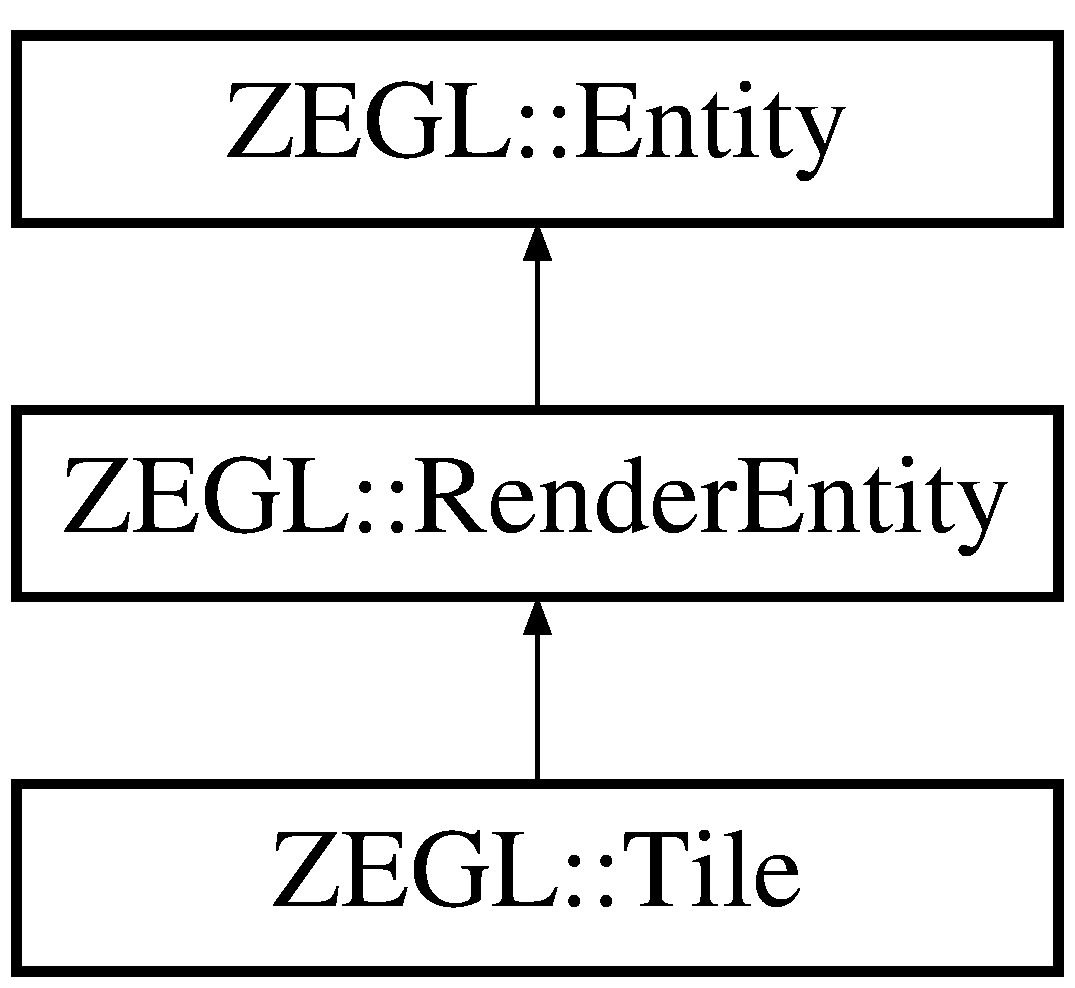
\includegraphics[height=3.000000cm]{class_z_e_g_l_1_1_entity}
\end{center}
\end{figure}
\subsection*{Public Member Functions}
\begin{DoxyCompactItemize}
\item 
\hypertarget{class_z_e_g_l_1_1_entity_a8011b8bee6e9c4893feb9a769db2a1d7}{}{\bfseries Entity} (const glm\+::vec3 \&pos=glm\+::vec3(0.\+0f), float rot=0.\+0f, float scale=1.\+0f)\label{class_z_e_g_l_1_1_entity_a8011b8bee6e9c4893feb9a769db2a1d7}

\item 
\hypertarget{class_z_e_g_l_1_1_entity_ab7136fc011809bc9bcc43862fd4c38ae}{}{\bfseries Entity} (const \hyperlink{class_z_e_g_l_1_1_entity}{Entity} \&entity)\label{class_z_e_g_l_1_1_entity_ab7136fc011809bc9bcc43862fd4c38ae}

\item 
\hypertarget{class_z_e_g_l_1_1_entity_ad5567bfde28b80800e34e17e8265cd26}{}void {\bfseries operator=} (\hyperlink{class_z_e_g_l_1_1_entity}{Entity} entity)\label{class_z_e_g_l_1_1_entity_ad5567bfde28b80800e34e17e8265cd26}

\item 
\hypertarget{class_z_e_g_l_1_1_entity_a39ceb0819b666f4605f3a6f78d4c7547}{}void {\bfseries Process\+Input} (const \hyperlink{class_z_e_g_l_1_1_input}{Input} \&input, float delta)\label{class_z_e_g_l_1_1_entity_a39ceb0819b666f4605f3a6f78d4c7547}

\item 
\hypertarget{class_z_e_g_l_1_1_entity_aa108f7618082d370fd414473a56ee61c}{}void {\bfseries Update} (float delta)\label{class_z_e_g_l_1_1_entity_aa108f7618082d370fd414473a56ee61c}

\item 
\hypertarget{class_z_e_g_l_1_1_entity_a026a323eaa1744bfaf4ff874d47abc2f}{}void {\bfseries Render} () const \label{class_z_e_g_l_1_1_entity_a026a323eaa1744bfaf4ff874d47abc2f}

\item 
\hypertarget{class_z_e_g_l_1_1_entity_a094aff78afc94ae73ca0bbc7f884e9b4}{}glm\+::vec3 {\bfseries Get\+Pos} () const \label{class_z_e_g_l_1_1_entity_a094aff78afc94ae73ca0bbc7f884e9b4}

\item 
\hypertarget{class_z_e_g_l_1_1_entity_acce32e7c26286c7309d05c4c6cc4a8e2}{}float {\bfseries Get\+Rot} () const \label{class_z_e_g_l_1_1_entity_acce32e7c26286c7309d05c4c6cc4a8e2}

\item 
\hypertarget{class_z_e_g_l_1_1_entity_ae74a51ca1aaac409c045be5511ada5c5}{}float {\bfseries Get\+Scale} () const \label{class_z_e_g_l_1_1_entity_ae74a51ca1aaac409c045be5511ada5c5}

\item 
\hypertarget{class_z_e_g_l_1_1_entity_af78fb1dfb0e5878802464486d0299348}{}void {\bfseries Set\+Pos} (float x, float y, float z=0.\+0f)\label{class_z_e_g_l_1_1_entity_af78fb1dfb0e5878802464486d0299348}

\item 
\hypertarget{class_z_e_g_l_1_1_entity_af41d770005e313b64e3141a5ca053076}{}void {\bfseries Set\+Pos} (const glm\+::vec3 \&pos)\label{class_z_e_g_l_1_1_entity_af41d770005e313b64e3141a5ca053076}

\item 
\hypertarget{class_z_e_g_l_1_1_entity_a1bb74f40f970621d73ffa40a46e54bbb}{}void {\bfseries Set\+Rot} (float rot)\label{class_z_e_g_l_1_1_entity_a1bb74f40f970621d73ffa40a46e54bbb}

\item 
\hypertarget{class_z_e_g_l_1_1_entity_ae3060c368e4fae9e3baec9147f5d5d84}{}void {\bfseries Set\+Scale} (float scale)\label{class_z_e_g_l_1_1_entity_ae3060c368e4fae9e3baec9147f5d5d84}

\item 
\hypertarget{class_z_e_g_l_1_1_entity_a656c356c7c35e01445ce543770c60e6f}{}const \hyperlink{struct_z_e_g_l_1_1_entity_data}{Entity\+Data} \& {\bfseries Get\+Data} () const \label{class_z_e_g_l_1_1_entity_a656c356c7c35e01445ce543770c60e6f}

\end{DoxyCompactItemize}
\subsection*{Protected Attributes}
\begin{DoxyCompactItemize}
\item 
\hypertarget{class_z_e_g_l_1_1_entity_a5f2e808fb78c9d7f4f16f755c4f598af}{}\hyperlink{struct_z_e_g_l_1_1_entity_data}{Entity\+Data} {\bfseries m\+\_\+data}\label{class_z_e_g_l_1_1_entity_a5f2e808fb78c9d7f4f16f755c4f598af}

\end{DoxyCompactItemize}


The documentation for this class was generated from the following files\+:\begin{DoxyCompactItemize}
\item 
include/entity.\+h\item 
src/entity.\+cpp\end{DoxyCompactItemize}

\hypertarget{struct_z_e_g_l_1_1_entity_data}{}\section{Z\+E\+G\+L\+:\+:Entity\+Data Struct Reference}
\label{struct_z_e_g_l_1_1_entity_data}\index{Z\+E\+G\+L\+::\+Entity\+Data@{Z\+E\+G\+L\+::\+Entity\+Data}}
\subsection*{Public Attributes}
\begin{DoxyCompactItemize}
\item 
\hypertarget{struct_z_e_g_l_1_1_entity_data_a766627340a91bddd339100545e291889}{}glm\+::vec3 {\bfseries m\+\_\+pos}\label{struct_z_e_g_l_1_1_entity_data_a766627340a91bddd339100545e291889}

\item 
\hypertarget{struct_z_e_g_l_1_1_entity_data_a315c1d6c3498bdd281c8bf76bd245b1c}{}float {\bfseries m\+\_\+rot}\label{struct_z_e_g_l_1_1_entity_data_a315c1d6c3498bdd281c8bf76bd245b1c}

\item 
\hypertarget{struct_z_e_g_l_1_1_entity_data_aafb6c681a1798a8ba567eb59c171d1ca}{}float {\bfseries m\+\_\+scale}\label{struct_z_e_g_l_1_1_entity_data_aafb6c681a1798a8ba567eb59c171d1ca}

\item 
\hypertarget{struct_z_e_g_l_1_1_entity_data_a02c43242c9cfc0edbd162f172c806380}{}glm\+::vec2 {\bfseries m\+\_\+tex\+Coords} \mbox{[}4\mbox{]}\label{struct_z_e_g_l_1_1_entity_data_a02c43242c9cfc0edbd162f172c806380}

\end{DoxyCompactItemize}


The documentation for this struct was generated from the following file\+:\begin{DoxyCompactItemize}
\item 
include/entity.\+h\end{DoxyCompactItemize}

\hypertarget{class_z_e_g_l_1_1_game}{}\section{Z\+E\+G\+L\+:\+:Game Class Reference}
\label{class_z_e_g_l_1_1_game}\index{Z\+E\+G\+L\+::\+Game@{Z\+E\+G\+L\+::\+Game}}


{\ttfamily \#include $<$game.\+h$>$}

\subsection*{Public Member Functions}
\begin{DoxyCompactItemize}
\item 
void \hyperlink{class_z_e_g_l_1_1_game_a08afc15e9896fef7f294f90d736d24cd}{Init} (const \hyperlink{class_z_e_g_l_1_1_window}{Window} $\ast$window)
\item 
void \hyperlink{class_z_e_g_l_1_1_game_ab64891eae2c4eb4f3bf7d161c6d5e37a}{Process\+Input} (const \hyperlink{class_z_e_g_l_1_1_input}{Input} \&input, float delta)
\item 
void \hyperlink{class_z_e_g_l_1_1_game_a6ad207394e4ce91f909d49c87802da08}{Update} (float delta)
\item 
void \hyperlink{class_z_e_g_l_1_1_game_a0897730fc9fed789f6c0f11d21a0c14a}{Render} ()
\item 
void \hyperlink{class_z_e_g_l_1_1_game_a38773e42c90201c4d8ca079ce54c4402}{Set\+F\+P\+S\+Display} (int frames)
\item 
const \hyperlink{class_z_e_g_l_1_1_light}{Light} $\ast$ \hyperlink{class_z_e_g_l_1_1_game_a82f5be49774c3ad1a96daac71eb0ddec}{Get\+Active\+Light} () const 
\item 
const \hyperlink{class_z_e_g_l_1_1_camera}{Camera} \& \hyperlink{class_z_e_g_l_1_1_game_a65c6ec575fef37dd386fa0534f6cad86}{Get\+Camera} () const 
\item 
const glm\+::vec4 \& \hyperlink{class_z_e_g_l_1_1_game_a82963ff86de3c1a1969f32de12c3863e}{Get\+Ambient\+Color} () const 
\item 
float \hyperlink{class_z_e_g_l_1_1_game_adb8a60aa109a04a92c3aee2065f79702}{Get\+Ambient\+Intensity} () const 
\item 
const \hyperlink{class_z_e_g_l_1_1_window}{Window} $\ast$ \hyperlink{class_z_e_g_l_1_1_game_a12474b22720b2559db897cd83b7dffce}{Get\+Window} ()
\end{DoxyCompactItemize}
\subsection*{Protected Attributes}
\begin{DoxyCompactItemize}
\item 
\hyperlink{class_z_e_g_l_1_1_camera}{Camera} $\ast$ \hyperlink{class_z_e_g_l_1_1_game_a75bf1aabc1dc5ad273611618c3ee05cf}{m\+\_\+camera}
\item 
const \hyperlink{class_z_e_g_l_1_1_window}{Window} $\ast$ \hyperlink{class_z_e_g_l_1_1_game_a72107b2460cfd896337dab847801fc1c}{m\+\_\+window}
\item 
glm\+::vec4 \hyperlink{class_z_e_g_l_1_1_game_a79bbd0830a4ac01cc820ba5a9bd26cd6}{m\+\_\+ambient\+Color}
\item 
const \hyperlink{class_z_e_g_l_1_1_light}{Light} $\ast$ \hyperlink{class_z_e_g_l_1_1_game_aa8ac2fd79809c3ad3477a4d723a7ae10}{m\+\_\+active\+Light}
\item 
std\+::vector$<$ \hyperlink{class_z_e_g_l_1_1_light}{Light} $\ast$ $>$ \hyperlink{class_z_e_g_l_1_1_game_ab301928901efd034fe40d53cdb54caf5}{m\+\_\+lights}
\item 
F\+O\+N\+Scontext $\ast$ \hyperlink{class_z_e_g_l_1_1_game_ab7239deb1a14053ae2d757994f2211d0}{m\+\_\+font\+Context}
\item 
char \hyperlink{class_z_e_g_l_1_1_game_ab290dd46ec4ff766bd56d0e3013bace1}{m\+\_\+fps} \mbox{[}16\mbox{]}
\end{DoxyCompactItemize}


\subsection{Detailed Description}
Base game class

This class is enough to run on its own and could be modified in to a full game. However, the intended use is that it is not used directly and is instead inherited from to create a new class for each project. The game class would be where all game-\/play related systems/objects reside e.\+g levels, fonts, entities. Then each can be updated and rendered in the respective \hyperlink{class_z_e_g_l_1_1_game_a6ad207394e4ce91f909d49c87802da08}{Update()} and \hyperlink{class_z_e_g_l_1_1_game_a0897730fc9fed789f6c0f11d21a0c14a}{Render()} funtions of the inherited game class. 

\subsection{Member Function Documentation}
\hypertarget{class_z_e_g_l_1_1_game_a82f5be49774c3ad1a96daac71eb0ddec}{}\index{Z\+E\+G\+L\+::\+Game@{Z\+E\+G\+L\+::\+Game}!Get\+Active\+Light@{Get\+Active\+Light}}
\index{Get\+Active\+Light@{Get\+Active\+Light}!Z\+E\+G\+L\+::\+Game@{Z\+E\+G\+L\+::\+Game}}
\subsubsection[{Get\+Active\+Light}]{\setlength{\rightskip}{0pt plus 5cm}const {\bf Light}$\ast$ Z\+E\+G\+L\+::\+Game\+::\+Get\+Active\+Light (
\begin{DoxyParamCaption}
{}
\end{DoxyParamCaption}
) const\hspace{0.3cm}{\ttfamily [inline]}}\label{class_z_e_g_l_1_1_game_a82f5be49774c3ad1a96daac71eb0ddec}
Get the currently active light.

\begin{DoxyReturn}{Returns}
Pointer to the currently active light (can be nullptr)
\end{DoxyReturn}
\begin{DoxySeeAlso}{See also}
\mbox{[}\hyperlink{class_z_e_g_l_1_1_light}{Light}\mbox{]} 
\end{DoxySeeAlso}
\hypertarget{class_z_e_g_l_1_1_game_a82963ff86de3c1a1969f32de12c3863e}{}\index{Z\+E\+G\+L\+::\+Game@{Z\+E\+G\+L\+::\+Game}!Get\+Ambient\+Color@{Get\+Ambient\+Color}}
\index{Get\+Ambient\+Color@{Get\+Ambient\+Color}!Z\+E\+G\+L\+::\+Game@{Z\+E\+G\+L\+::\+Game}}
\subsubsection[{Get\+Ambient\+Color}]{\setlength{\rightskip}{0pt plus 5cm}const glm\+::vec4\& Z\+E\+G\+L\+::\+Game\+::\+Get\+Ambient\+Color (
\begin{DoxyParamCaption}
{}
\end{DoxyParamCaption}
) const\hspace{0.3cm}{\ttfamily [inline]}}\label{class_z_e_g_l_1_1_game_a82963ff86de3c1a1969f32de12c3863e}
Get the ambient color for the \hyperlink{class_z_e_g_l_1_1_game}{Game} environment.

\begin{DoxyReturn}{Returns}
A glm\+::vec4 using r,g,b as color and a as intensity 
\end{DoxyReturn}
\hypertarget{class_z_e_g_l_1_1_game_adb8a60aa109a04a92c3aee2065f79702}{}\index{Z\+E\+G\+L\+::\+Game@{Z\+E\+G\+L\+::\+Game}!Get\+Ambient\+Intensity@{Get\+Ambient\+Intensity}}
\index{Get\+Ambient\+Intensity@{Get\+Ambient\+Intensity}!Z\+E\+G\+L\+::\+Game@{Z\+E\+G\+L\+::\+Game}}
\subsubsection[{Get\+Ambient\+Intensity}]{\setlength{\rightskip}{0pt plus 5cm}float Z\+E\+G\+L\+::\+Game\+::\+Get\+Ambient\+Intensity (
\begin{DoxyParamCaption}
{}
\end{DoxyParamCaption}
) const\hspace{0.3cm}{\ttfamily [inline]}}\label{class_z_e_g_l_1_1_game_adb8a60aa109a04a92c3aee2065f79702}
Get the ambient intensity for the \hyperlink{class_z_e_g_l_1_1_game}{Game} environment.

\begin{DoxyReturn}{Returns}
Just the alpha component of m\+\_\+ambient\+Color 
\end{DoxyReturn}
\hypertarget{class_z_e_g_l_1_1_game_a65c6ec575fef37dd386fa0534f6cad86}{}\index{Z\+E\+G\+L\+::\+Game@{Z\+E\+G\+L\+::\+Game}!Get\+Camera@{Get\+Camera}}
\index{Get\+Camera@{Get\+Camera}!Z\+E\+G\+L\+::\+Game@{Z\+E\+G\+L\+::\+Game}}
\subsubsection[{Get\+Camera}]{\setlength{\rightskip}{0pt plus 5cm}const {\bf Camera}\& Z\+E\+G\+L\+::\+Game\+::\+Get\+Camera (
\begin{DoxyParamCaption}
{}
\end{DoxyParamCaption}
) const\hspace{0.3cm}{\ttfamily [inline]}}\label{class_z_e_g_l_1_1_game_a65c6ec575fef37dd386fa0534f6cad86}
Get the \hyperlink{class_z_e_g_l_1_1_game}{Game} \hyperlink{class_z_e_g_l_1_1_camera}{Camera}.

\begin{DoxyReturn}{Returns}
The \hyperlink{class_z_e_g_l_1_1_camera}{Camera} being used by the game for display calculations
\end{DoxyReturn}
\begin{DoxySeeAlso}{See also}
\mbox{[}\hyperlink{class_z_e_g_l_1_1_camera}{Camera}\mbox{]} 
\end{DoxySeeAlso}
\hypertarget{class_z_e_g_l_1_1_game_a12474b22720b2559db897cd83b7dffce}{}\index{Z\+E\+G\+L\+::\+Game@{Z\+E\+G\+L\+::\+Game}!Get\+Window@{Get\+Window}}
\index{Get\+Window@{Get\+Window}!Z\+E\+G\+L\+::\+Game@{Z\+E\+G\+L\+::\+Game}}
\subsubsection[{Get\+Window}]{\setlength{\rightskip}{0pt plus 5cm}const {\bf Window}$\ast$ Z\+E\+G\+L\+::\+Game\+::\+Get\+Window (
\begin{DoxyParamCaption}
{}
\end{DoxyParamCaption}
)\hspace{0.3cm}{\ttfamily [inline]}}\label{class_z_e_g_l_1_1_game_a12474b22720b2559db897cd83b7dffce}
Get the game \hyperlink{class_z_e_g_l_1_1_window}{Window}.

\begin{DoxyReturn}{Returns}
Pointer to the \hyperlink{class_z_e_g_l_1_1_window}{Window} being used by the \hyperlink{class_z_e_g_l_1_1_game}{Game} for rendering
\end{DoxyReturn}
\begin{DoxySeeAlso}{See also}
\mbox{[}\hyperlink{class_z_e_g_l_1_1_window}{Window}\mbox{]} 
\end{DoxySeeAlso}
\hypertarget{class_z_e_g_l_1_1_game_a08afc15e9896fef7f294f90d736d24cd}{}\index{Z\+E\+G\+L\+::\+Game@{Z\+E\+G\+L\+::\+Game}!Init@{Init}}
\index{Init@{Init}!Z\+E\+G\+L\+::\+Game@{Z\+E\+G\+L\+::\+Game}}
\subsubsection[{Init}]{\setlength{\rightskip}{0pt plus 5cm}void Game\+::\+Init (
\begin{DoxyParamCaption}
\item[{const {\bf Window} $\ast$}]{window}
\end{DoxyParamCaption}
)}\label{class_z_e_g_l_1_1_game_a08afc15e9896fef7f294f90d736d24cd}
All resource loading, game related initialization and Open\+G\+L rendering configuration is performed here.


\begin{DoxyParams}[1]{Parameters}
\mbox{\tt in}  & {\em window} & Pointer to an already created \hyperlink{class_z_e_g_l_1_1_window}{Window} \\
\hline
\end{DoxyParams}
\begin{DoxySeeAlso}{See also}
\mbox{[}\hyperlink{class_z_e_g_l_1_1_window}{Window}\mbox{]} 
\end{DoxySeeAlso}
\hypertarget{class_z_e_g_l_1_1_game_ab64891eae2c4eb4f3bf7d161c6d5e37a}{}\index{Z\+E\+G\+L\+::\+Game@{Z\+E\+G\+L\+::\+Game}!Process\+Input@{Process\+Input}}
\index{Process\+Input@{Process\+Input}!Z\+E\+G\+L\+::\+Game@{Z\+E\+G\+L\+::\+Game}}
\subsubsection[{Process\+Input}]{\setlength{\rightskip}{0pt plus 5cm}void Game\+::\+Process\+Input (
\begin{DoxyParamCaption}
\item[{const {\bf Input} \&}]{input, }
\item[{float}]{delta}
\end{DoxyParamCaption}
)}\label{class_z_e_g_l_1_1_game_ab64891eae2c4eb4f3bf7d161c6d5e37a}
Any user input will be registered and actioned here.


\begin{DoxyParams}[1]{Parameters}
\mbox{\tt in}  & {\em input} & \hyperlink{class_z_e_g_l_1_1_input}{Input} class which is managing the user input \\
\hline
\mbox{\tt in}  & {\em delta} & Delta frame time in milliseconds\\
\hline
\end{DoxyParams}
\begin{DoxyWarning}{Warning}
To ensure input is handled correctly this function must be called after Window\+::\+Update() but before \hyperlink{class_z_e_g_l_1_1_game_a6ad207394e4ce91f909d49c87802da08}{Game\+::\+Update()}.
\end{DoxyWarning}
\begin{DoxySeeAlso}{See also}
\mbox{[}\hyperlink{class_z_e_g_l_1_1_input}{Input}\mbox{]}\mbox{[}\hyperlink{class_z_e_g_l_1_1_window}{Window}\mbox{]} 
\end{DoxySeeAlso}
\hypertarget{class_z_e_g_l_1_1_game_a0897730fc9fed789f6c0f11d21a0c14a}{}\index{Z\+E\+G\+L\+::\+Game@{Z\+E\+G\+L\+::\+Game}!Render@{Render}}
\index{Render@{Render}!Z\+E\+G\+L\+::\+Game@{Z\+E\+G\+L\+::\+Game}}
\subsubsection[{Render}]{\setlength{\rightskip}{0pt plus 5cm}void Game\+::\+Render (
\begin{DoxyParamCaption}
{}
\end{DoxyParamCaption}
)}\label{class_z_e_g_l_1_1_game_a0897730fc9fed789f6c0f11d21a0c14a}
Render all objects and swap the buffers to display to the screen. \hypertarget{class_z_e_g_l_1_1_game_a38773e42c90201c4d8ca079ce54c4402}{}\index{Z\+E\+G\+L\+::\+Game@{Z\+E\+G\+L\+::\+Game}!Set\+F\+P\+S\+Display@{Set\+F\+P\+S\+Display}}
\index{Set\+F\+P\+S\+Display@{Set\+F\+P\+S\+Display}!Z\+E\+G\+L\+::\+Game@{Z\+E\+G\+L\+::\+Game}}
\subsubsection[{Set\+F\+P\+S\+Display}]{\setlength{\rightskip}{0pt plus 5cm}void Game\+::\+Set\+F\+P\+S\+Display (
\begin{DoxyParamCaption}
\item[{int}]{frames}
\end{DoxyParamCaption}
)}\label{class_z_e_g_l_1_1_game_a38773e42c90201c4d8ca079ce54c4402}
Update the char array m\+\_\+fps to include the passed int value.


\begin{DoxyParams}[1]{Parameters}
\mbox{\tt in}  & {\em frames} & Current frame rate \\
\hline
\end{DoxyParams}
\hypertarget{class_z_e_g_l_1_1_game_a6ad207394e4ce91f909d49c87802da08}{}\index{Z\+E\+G\+L\+::\+Game@{Z\+E\+G\+L\+::\+Game}!Update@{Update}}
\index{Update@{Update}!Z\+E\+G\+L\+::\+Game@{Z\+E\+G\+L\+::\+Game}}
\subsubsection[{Update}]{\setlength{\rightskip}{0pt plus 5cm}void Game\+::\+Update (
\begin{DoxyParamCaption}
\item[{float}]{delta}
\end{DoxyParamCaption}
)}\label{class_z_e_g_l_1_1_game_a6ad207394e4ce91f909d49c87802da08}
Update all game objects using delta time step.


\begin{DoxyParams}[1]{Parameters}
\mbox{\tt in}  & {\em delta} & Delta frame time in milliseconds \\
\hline
\end{DoxyParams}


\subsection{Member Data Documentation}
\hypertarget{class_z_e_g_l_1_1_game_aa8ac2fd79809c3ad3477a4d723a7ae10}{}\index{Z\+E\+G\+L\+::\+Game@{Z\+E\+G\+L\+::\+Game}!m\+\_\+active\+Light@{m\+\_\+active\+Light}}
\index{m\+\_\+active\+Light@{m\+\_\+active\+Light}!Z\+E\+G\+L\+::\+Game@{Z\+E\+G\+L\+::\+Game}}
\subsubsection[{m\+\_\+active\+Light}]{\setlength{\rightskip}{0pt plus 5cm}const {\bf Light}$\ast$ Z\+E\+G\+L\+::\+Game\+::m\+\_\+active\+Light\hspace{0.3cm}{\ttfamily [protected]}}\label{class_z_e_g_l_1_1_game_aa8ac2fd79809c3ad3477a4d723a7ae10}
Pointer to the currently active \hyperlink{class_z_e_g_l_1_1_light}{Light} \hypertarget{class_z_e_g_l_1_1_game_a79bbd0830a4ac01cc820ba5a9bd26cd6}{}\index{Z\+E\+G\+L\+::\+Game@{Z\+E\+G\+L\+::\+Game}!m\+\_\+ambient\+Color@{m\+\_\+ambient\+Color}}
\index{m\+\_\+ambient\+Color@{m\+\_\+ambient\+Color}!Z\+E\+G\+L\+::\+Game@{Z\+E\+G\+L\+::\+Game}}
\subsubsection[{m\+\_\+ambient\+Color}]{\setlength{\rightskip}{0pt plus 5cm}glm\+::vec4 Z\+E\+G\+L\+::\+Game\+::m\+\_\+ambient\+Color\hspace{0.3cm}{\ttfamily [protected]}}\label{class_z_e_g_l_1_1_game_a79bbd0830a4ac01cc820ba5a9bd26cd6}
Ambient color for the world (used if there is no \hyperlink{class_z_e_g_l_1_1_light}{Light}) \hypertarget{class_z_e_g_l_1_1_game_a75bf1aabc1dc5ad273611618c3ee05cf}{}\index{Z\+E\+G\+L\+::\+Game@{Z\+E\+G\+L\+::\+Game}!m\+\_\+camera@{m\+\_\+camera}}
\index{m\+\_\+camera@{m\+\_\+camera}!Z\+E\+G\+L\+::\+Game@{Z\+E\+G\+L\+::\+Game}}
\subsubsection[{m\+\_\+camera}]{\setlength{\rightskip}{0pt plus 5cm}{\bf Camera}$\ast$ Z\+E\+G\+L\+::\+Game\+::m\+\_\+camera\hspace{0.3cm}{\ttfamily [protected]}}\label{class_z_e_g_l_1_1_game_a75bf1aabc1dc5ad273611618c3ee05cf}
The \hyperlink{class_z_e_g_l_1_1_game}{Game} \hyperlink{class_z_e_g_l_1_1_camera}{Camera} \hypertarget{class_z_e_g_l_1_1_game_ab7239deb1a14053ae2d757994f2211d0}{}\index{Z\+E\+G\+L\+::\+Game@{Z\+E\+G\+L\+::\+Game}!m\+\_\+font\+Context@{m\+\_\+font\+Context}}
\index{m\+\_\+font\+Context@{m\+\_\+font\+Context}!Z\+E\+G\+L\+::\+Game@{Z\+E\+G\+L\+::\+Game}}
\subsubsection[{m\+\_\+font\+Context}]{\setlength{\rightskip}{0pt plus 5cm}F\+O\+N\+Scontext$\ast$ Z\+E\+G\+L\+::\+Game\+::m\+\_\+font\+Context\hspace{0.3cm}{\ttfamily [protected]}}\label{class_z_e_g_l_1_1_game_ab7239deb1a14053ae2d757994f2211d0}
Cache of all fonts loaded -\/ request by int index \hypertarget{class_z_e_g_l_1_1_game_ab290dd46ec4ff766bd56d0e3013bace1}{}\index{Z\+E\+G\+L\+::\+Game@{Z\+E\+G\+L\+::\+Game}!m\+\_\+fps@{m\+\_\+fps}}
\index{m\+\_\+fps@{m\+\_\+fps}!Z\+E\+G\+L\+::\+Game@{Z\+E\+G\+L\+::\+Game}}
\subsubsection[{m\+\_\+fps}]{\setlength{\rightskip}{0pt plus 5cm}char Z\+E\+G\+L\+::\+Game\+::m\+\_\+fps\mbox{[}16\mbox{]}\hspace{0.3cm}{\ttfamily [protected]}}\label{class_z_e_g_l_1_1_game_ab290dd46ec4ff766bd56d0e3013bace1}
char array for displaying F\+P\+S string \hypertarget{class_z_e_g_l_1_1_game_ab301928901efd034fe40d53cdb54caf5}{}\index{Z\+E\+G\+L\+::\+Game@{Z\+E\+G\+L\+::\+Game}!m\+\_\+lights@{m\+\_\+lights}}
\index{m\+\_\+lights@{m\+\_\+lights}!Z\+E\+G\+L\+::\+Game@{Z\+E\+G\+L\+::\+Game}}
\subsubsection[{m\+\_\+lights}]{\setlength{\rightskip}{0pt plus 5cm}std\+::vector$<${\bf Light}$\ast$$>$ Z\+E\+G\+L\+::\+Game\+::m\+\_\+lights\hspace{0.3cm}{\ttfamily [protected]}}\label{class_z_e_g_l_1_1_game_ab301928901efd034fe40d53cdb54caf5}
Stores all the lights for the game \hypertarget{class_z_e_g_l_1_1_game_a72107b2460cfd896337dab847801fc1c}{}\index{Z\+E\+G\+L\+::\+Game@{Z\+E\+G\+L\+::\+Game}!m\+\_\+window@{m\+\_\+window}}
\index{m\+\_\+window@{m\+\_\+window}!Z\+E\+G\+L\+::\+Game@{Z\+E\+G\+L\+::\+Game}}
\subsubsection[{m\+\_\+window}]{\setlength{\rightskip}{0pt plus 5cm}const {\bf Window}$\ast$ Z\+E\+G\+L\+::\+Game\+::m\+\_\+window\hspace{0.3cm}{\ttfamily [protected]}}\label{class_z_e_g_l_1_1_game_a72107b2460cfd896337dab847801fc1c}
The \hyperlink{class_z_e_g_l_1_1_window}{Window} used for rendering 

The documentation for this class was generated from the following files\+:\begin{DoxyCompactItemize}
\item 
include/game.\+h\item 
src/game.\+cpp\end{DoxyCompactItemize}

\hypertarget{class_z_e_g_l_1_1_input}{}\section{Z\+E\+G\+L\+:\+:Input Class Reference}
\label{class_z_e_g_l_1_1_input}\index{Z\+E\+G\+L\+::\+Input@{Z\+E\+G\+L\+::\+Input}}
\subsection*{Public Types}
\begin{DoxyCompactItemize}
\item 
\hypertarget{class_z_e_g_l_1_1_input_aa767ce6639ffad5eb032a94b3c423b9a}{}enum \{ \\*
{\bfseries M\+O\+U\+S\+E\+\_\+\+L\+E\+F\+T\+\_\+\+B\+U\+T\+T\+O\+N} = 1, 
{\bfseries M\+O\+U\+S\+E\+\_\+\+M\+I\+D\+D\+L\+E\+\_\+\+B\+U\+T\+T\+O\+N} = 2, 
{\bfseries M\+O\+U\+S\+E\+\_\+\+R\+I\+G\+H\+T\+\_\+\+B\+U\+T\+T\+O\+N} = 3, 
{\bfseries M\+O\+U\+S\+E\+\_\+\+W\+H\+E\+E\+L\+\_\+\+U\+P} = 4, 
\\*
{\bfseries M\+O\+U\+S\+E\+\_\+\+W\+H\+E\+E\+L\+\_\+\+D\+O\+W\+N} = 5, 
{\bfseries M\+A\+X\+\_\+\+M\+O\+U\+S\+E\+\_\+\+B\+U\+T\+T\+O\+N\+S}
 \}\label{class_z_e_g_l_1_1_input_aa767ce6639ffad5eb032a94b3c423b9a}

\item 
\hypertarget{class_z_e_g_l_1_1_input_a63c4a9987b2fe681fcf8e17d5f88a838}{}enum \{ \\*
{\bfseries K\+E\+Y\+\_\+\+U\+N\+K\+N\+O\+W\+N} = 0, 
{\bfseries K\+E\+Y\+\_\+\+A} = 4, 
{\bfseries K\+E\+Y\+\_\+\+B} = 5, 
{\bfseries K\+E\+Y\+\_\+\+C} = 6, 
\\*
{\bfseries K\+E\+Y\+\_\+\+D} = 7, 
{\bfseries K\+E\+Y\+\_\+\+E} = 8, 
{\bfseries K\+E\+Y\+\_\+\+F} = 9, 
{\bfseries K\+E\+Y\+\_\+\+G} = 10, 
\\*
{\bfseries K\+E\+Y\+\_\+\+H} = 11, 
{\bfseries K\+E\+Y\+\_\+\+I} = 12, 
{\bfseries K\+E\+Y\+\_\+\+J} = 13, 
{\bfseries K\+E\+Y\+\_\+\+K} = 14, 
\\*
{\bfseries K\+E\+Y\+\_\+\+L} = 15, 
{\bfseries K\+E\+Y\+\_\+\+M} = 16, 
{\bfseries K\+E\+Y\+\_\+\+N} = 17, 
{\bfseries K\+E\+Y\+\_\+\+O} = 18, 
\\*
{\bfseries K\+E\+Y\+\_\+\+P} = 19, 
{\bfseries K\+E\+Y\+\_\+\+Q} = 20, 
{\bfseries K\+E\+Y\+\_\+\+R} = 21, 
{\bfseries K\+E\+Y\+\_\+\+S} = 22, 
\\*
{\bfseries K\+E\+Y\+\_\+\+T} = 23, 
{\bfseries K\+E\+Y\+\_\+\+U} = 24, 
{\bfseries K\+E\+Y\+\_\+\+V} = 25, 
{\bfseries K\+E\+Y\+\_\+\+W} = 26, 
\\*
{\bfseries K\+E\+Y\+\_\+\+X} = 27, 
{\bfseries K\+E\+Y\+\_\+\+Y} = 28, 
{\bfseries K\+E\+Y\+\_\+\+Z} = 29, 
{\bfseries K\+E\+Y\+\_\+1} = 30, 
\\*
{\bfseries K\+E\+Y\+\_\+2} = 31, 
{\bfseries K\+E\+Y\+\_\+3} = 32, 
{\bfseries K\+E\+Y\+\_\+4} = 33, 
{\bfseries K\+E\+Y\+\_\+5} = 34, 
\\*
{\bfseries K\+E\+Y\+\_\+6} = 35, 
{\bfseries K\+E\+Y\+\_\+7} = 36, 
{\bfseries K\+E\+Y\+\_\+8} = 37, 
{\bfseries K\+E\+Y\+\_\+9} = 38, 
\\*
{\bfseries K\+E\+Y\+\_\+0} = 39, 
{\bfseries K\+E\+Y\+\_\+\+R\+E\+T\+U\+R\+N} = 40, 
{\bfseries K\+E\+Y\+\_\+\+E\+S\+C\+A\+P\+E} = 41, 
{\bfseries K\+E\+Y\+\_\+\+B\+A\+C\+K\+S\+P\+A\+C\+E} = 42, 
\\*
{\bfseries K\+E\+Y\+\_\+\+T\+A\+B} = 43, 
{\bfseries K\+E\+Y\+\_\+\+S\+P\+A\+C\+E} = 44, 
{\bfseries K\+E\+Y\+\_\+\+M\+I\+N\+U\+S} = 45, 
{\bfseries K\+E\+Y\+\_\+\+E\+Q\+U\+A\+L\+S} = 46, 
\\*
{\bfseries K\+E\+Y\+\_\+\+L\+E\+F\+T\+B\+R\+A\+C\+K\+E\+T} = 47, 
{\bfseries K\+E\+Y\+\_\+\+R\+I\+G\+H\+T\+B\+R\+A\+C\+K\+E\+T} = 48, 
{\bfseries K\+E\+Y\+\_\+\+B\+A\+C\+K\+S\+L\+A\+S\+H} = 49, 
{\bfseries K\+E\+Y\+\_\+\+N\+O\+N\+U\+S\+H\+A\+S\+H} = 50, 
\\*
{\bfseries K\+E\+Y\+\_\+\+S\+E\+M\+I\+C\+O\+L\+O\+N} = 51, 
{\bfseries K\+E\+Y\+\_\+\+A\+P\+O\+S\+T\+R\+O\+P\+H\+E} = 52, 
{\bfseries K\+E\+Y\+\_\+\+G\+R\+A\+V\+E} = 53, 
{\bfseries K\+E\+Y\+\_\+\+C\+O\+M\+M\+A} = 54, 
\\*
{\bfseries K\+E\+Y\+\_\+\+P\+E\+R\+I\+O\+D} = 55, 
{\bfseries K\+E\+Y\+\_\+\+S\+L\+A\+S\+H} = 56, 
{\bfseries K\+E\+Y\+\_\+\+C\+A\+P\+S\+L\+O\+C\+K} = 57, 
{\bfseries K\+E\+Y\+\_\+\+F1} = 58, 
\\*
{\bfseries K\+E\+Y\+\_\+\+F2} = 59, 
{\bfseries K\+E\+Y\+\_\+\+F3} = 60, 
{\bfseries K\+E\+Y\+\_\+\+F4} = 61, 
{\bfseries K\+E\+Y\+\_\+\+F5} = 62, 
\\*
{\bfseries K\+E\+Y\+\_\+\+F6} = 63, 
{\bfseries K\+E\+Y\+\_\+\+F7} = 64, 
{\bfseries K\+E\+Y\+\_\+\+F8} = 65, 
{\bfseries K\+E\+Y\+\_\+\+F9} = 66, 
\\*
{\bfseries K\+E\+Y\+\_\+\+F10} = 67, 
{\bfseries K\+E\+Y\+\_\+\+F11} = 68, 
{\bfseries K\+E\+Y\+\_\+\+F12} = 69, 
{\bfseries K\+E\+Y\+\_\+\+P\+R\+I\+N\+T\+S\+C\+R\+E\+E\+N} = 70, 
\\*
{\bfseries K\+E\+Y\+\_\+\+S\+C\+R\+O\+L\+L\+L\+O\+C\+K} = 71, 
{\bfseries K\+E\+Y\+\_\+\+P\+A\+U\+S\+E} = 72, 
{\bfseries K\+E\+Y\+\_\+\+I\+N\+S\+E\+R\+T} = 73, 
{\bfseries K\+E\+Y\+\_\+\+H\+O\+M\+E} = 74, 
\\*
{\bfseries K\+E\+Y\+\_\+\+P\+A\+G\+E\+U\+P} = 75, 
{\bfseries K\+E\+Y\+\_\+\+D\+E\+L\+E\+T\+E} = 76, 
{\bfseries K\+E\+Y\+\_\+\+E\+N\+D} = 77, 
{\bfseries K\+E\+Y\+\_\+\+P\+A\+G\+E\+D\+O\+W\+N} = 78, 
\\*
{\bfseries K\+E\+Y\+\_\+\+R\+I\+G\+H\+T} = 79, 
{\bfseries K\+E\+Y\+\_\+\+L\+E\+F\+T} = 80, 
{\bfseries K\+E\+Y\+\_\+\+D\+O\+W\+N} = 81, 
{\bfseries K\+E\+Y\+\_\+\+U\+P} = 82, 
\\*
{\bfseries K\+E\+Y\+\_\+\+N\+U\+M\+L\+O\+C\+K\+C\+L\+E\+A\+R} = 83, 
{\bfseries K\+E\+Y\+\_\+\+K\+P\+\_\+\+D\+I\+V\+I\+D\+E} = 84, 
{\bfseries K\+E\+Y\+\_\+\+K\+P\+\_\+\+M\+U\+L\+T\+I\+P\+L\+Y} = 85, 
{\bfseries K\+E\+Y\+\_\+\+K\+P\+\_\+\+M\+I\+N\+U\+S} = 86, 
\\*
{\bfseries K\+E\+Y\+\_\+\+K\+P\+\_\+\+P\+L\+U\+S} = 87, 
{\bfseries K\+E\+Y\+\_\+\+K\+P\+\_\+\+E\+N\+T\+E\+R} = 88, 
{\bfseries K\+E\+Y\+\_\+\+K\+P\+\_\+1} = 89, 
{\bfseries K\+E\+Y\+\_\+\+K\+P\+\_\+2} = 90, 
\\*
{\bfseries K\+E\+Y\+\_\+\+K\+P\+\_\+3} = 91, 
{\bfseries K\+E\+Y\+\_\+\+K\+P\+\_\+4} = 92, 
{\bfseries K\+E\+Y\+\_\+\+K\+P\+\_\+5} = 93, 
{\bfseries K\+E\+Y\+\_\+\+K\+P\+\_\+6} = 94, 
\\*
{\bfseries K\+E\+Y\+\_\+\+K\+P\+\_\+7} = 95, 
{\bfseries K\+E\+Y\+\_\+\+K\+P\+\_\+8} = 96, 
{\bfseries K\+E\+Y\+\_\+\+K\+P\+\_\+9} = 97, 
{\bfseries K\+E\+Y\+\_\+\+K\+P\+\_\+0} = 98, 
\\*
{\bfseries K\+E\+Y\+\_\+\+K\+P\+\_\+\+P\+E\+R\+I\+O\+D} = 99, 
{\bfseries K\+E\+Y\+\_\+\+N\+O\+N\+U\+S\+B\+A\+C\+K\+S\+L\+A\+S\+H} = 100, 
{\bfseries K\+E\+Y\+\_\+\+A\+P\+P\+L\+I\+C\+A\+T\+I\+O\+N} = 101, 
{\bfseries K\+E\+Y\+\_\+\+P\+O\+W\+E\+R} = 102, 
\\*
{\bfseries K\+E\+Y\+\_\+\+K\+P\+\_\+\+E\+Q\+U\+A\+L\+S} = 103, 
{\bfseries K\+E\+Y\+\_\+\+F13} = 104, 
{\bfseries K\+E\+Y\+\_\+\+F14} = 105, 
{\bfseries K\+E\+Y\+\_\+\+F15} = 106, 
\\*
{\bfseries K\+E\+Y\+\_\+\+F16} = 107, 
{\bfseries K\+E\+Y\+\_\+\+F17} = 108, 
{\bfseries K\+E\+Y\+\_\+\+F18} = 109, 
{\bfseries K\+E\+Y\+\_\+\+F19} = 110, 
\\*
{\bfseries K\+E\+Y\+\_\+\+F20} = 111, 
{\bfseries K\+E\+Y\+\_\+\+F21} = 112, 
{\bfseries K\+E\+Y\+\_\+\+F22} = 113, 
{\bfseries K\+E\+Y\+\_\+\+F23} = 114, 
\\*
{\bfseries K\+E\+Y\+\_\+\+F24} = 115, 
{\bfseries K\+E\+Y\+\_\+\+E\+X\+E\+C\+U\+T\+E} = 116, 
{\bfseries K\+E\+Y\+\_\+\+H\+E\+L\+P} = 117, 
{\bfseries K\+E\+Y\+\_\+\+M\+E\+N\+U} = 118, 
\\*
{\bfseries K\+E\+Y\+\_\+\+S\+E\+L\+E\+C\+T} = 119, 
{\bfseries K\+E\+Y\+\_\+\+S\+T\+O\+P} = 120, 
{\bfseries K\+E\+Y\+\_\+\+A\+G\+A\+I\+N} = 121, 
{\bfseries K\+E\+Y\+\_\+\+U\+N\+D\+O} = 122, 
\\*
{\bfseries K\+E\+Y\+\_\+\+C\+U\+T} = 123, 
{\bfseries K\+E\+Y\+\_\+\+C\+O\+P\+Y} = 124, 
{\bfseries K\+E\+Y\+\_\+\+P\+A\+S\+T\+E} = 125, 
{\bfseries K\+E\+Y\+\_\+\+F\+I\+N\+D} = 126, 
\\*
{\bfseries K\+E\+Y\+\_\+\+M\+U\+T\+E} = 127, 
{\bfseries K\+E\+Y\+\_\+\+V\+O\+L\+U\+M\+E\+U\+P} = 128, 
{\bfseries K\+E\+Y\+\_\+\+V\+O\+L\+U\+M\+E\+D\+O\+W\+N} = 129, 
{\bfseries K\+E\+Y\+\_\+\+K\+P\+\_\+\+C\+O\+M\+M\+A} = 133, 
\\*
{\bfseries K\+E\+Y\+\_\+\+K\+P\+\_\+\+E\+Q\+U\+A\+L\+S\+A\+S400} = 134, 
{\bfseries K\+E\+Y\+\_\+\+A\+L\+T\+E\+R\+A\+S\+E} = 153, 
{\bfseries K\+E\+Y\+\_\+\+S\+Y\+S\+R\+E\+Q} = 154, 
{\bfseries K\+E\+Y\+\_\+\+C\+A\+N\+C\+E\+L} = 155, 
\\*
{\bfseries K\+E\+Y\+\_\+\+C\+L\+E\+A\+R} = 156, 
{\bfseries K\+E\+Y\+\_\+\+P\+R\+I\+O\+R} = 157, 
{\bfseries K\+E\+Y\+\_\+\+R\+E\+T\+U\+R\+N2} = 158, 
{\bfseries K\+E\+Y\+\_\+\+S\+E\+P\+A\+R\+A\+T\+O\+R} = 159, 
\\*
{\bfseries K\+E\+Y\+\_\+\+O\+U\+T} = 160, 
{\bfseries K\+E\+Y\+\_\+\+O\+P\+E\+R} = 161, 
{\bfseries K\+E\+Y\+\_\+\+C\+L\+E\+A\+R\+A\+G\+A\+I\+N} = 162, 
{\bfseries K\+E\+Y\+\_\+\+C\+R\+S\+E\+L} = 163, 
\\*
{\bfseries K\+E\+Y\+\_\+\+E\+X\+S\+E\+L} = 164, 
{\bfseries K\+E\+Y\+\_\+\+K\+P\+\_\+00} = 176, 
{\bfseries K\+E\+Y\+\_\+\+K\+P\+\_\+000} = 177, 
{\bfseries K\+E\+Y\+\_\+\+T\+H\+O\+U\+S\+A\+N\+D\+S\+S\+E\+P\+A\+R\+A\+T\+O\+R} = 178, 
\\*
{\bfseries K\+E\+Y\+\_\+\+D\+E\+C\+I\+M\+A\+L\+S\+E\+P\+A\+R\+A\+T\+O\+R} = 179, 
{\bfseries K\+E\+Y\+\_\+\+C\+U\+R\+R\+E\+N\+C\+Y\+U\+N\+I\+T} = 180, 
{\bfseries K\+E\+Y\+\_\+\+C\+U\+R\+R\+E\+N\+C\+Y\+S\+U\+B\+U\+N\+I\+T} = 181, 
{\bfseries K\+E\+Y\+\_\+\+K\+P\+\_\+\+L\+E\+F\+T\+P\+A\+R\+E\+N} = 182, 
\\*
{\bfseries K\+E\+Y\+\_\+\+K\+P\+\_\+\+R\+I\+G\+H\+T\+P\+A\+R\+E\+N} = 183, 
{\bfseries K\+E\+Y\+\_\+\+K\+P\+\_\+\+L\+E\+F\+T\+B\+R\+A\+C\+E} = 184, 
{\bfseries K\+E\+Y\+\_\+\+K\+P\+\_\+\+R\+I\+G\+H\+T\+B\+R\+A\+C\+E} = 185, 
{\bfseries K\+E\+Y\+\_\+\+K\+P\+\_\+\+T\+A\+B} = 186, 
\\*
{\bfseries K\+E\+Y\+\_\+\+K\+P\+\_\+\+B\+A\+C\+K\+S\+P\+A\+C\+E} = 187, 
{\bfseries K\+E\+Y\+\_\+\+K\+P\+\_\+\+A} = 188, 
{\bfseries K\+E\+Y\+\_\+\+K\+P\+\_\+\+B} = 189, 
{\bfseries K\+E\+Y\+\_\+\+K\+P\+\_\+\+C} = 190, 
\\*
{\bfseries K\+E\+Y\+\_\+\+K\+P\+\_\+\+D} = 191, 
{\bfseries K\+E\+Y\+\_\+\+K\+P\+\_\+\+E} = 192, 
{\bfseries K\+E\+Y\+\_\+\+K\+P\+\_\+\+F} = 193, 
{\bfseries K\+E\+Y\+\_\+\+K\+P\+\_\+\+X\+O\+R} = 194, 
\\*
{\bfseries K\+E\+Y\+\_\+\+K\+P\+\_\+\+P\+O\+W\+E\+R} = 195, 
{\bfseries K\+E\+Y\+\_\+\+K\+P\+\_\+\+P\+E\+R\+C\+E\+N\+T} = 196, 
{\bfseries K\+E\+Y\+\_\+\+K\+P\+\_\+\+L\+E\+S\+S} = 197, 
{\bfseries K\+E\+Y\+\_\+\+K\+P\+\_\+\+G\+R\+E\+A\+T\+E\+R} = 198, 
\\*
{\bfseries K\+E\+Y\+\_\+\+K\+P\+\_\+\+A\+M\+P\+E\+R\+S\+A\+N\+D} = 199, 
{\bfseries K\+E\+Y\+\_\+\+K\+P\+\_\+\+D\+B\+L\+A\+M\+P\+E\+R\+S\+A\+N\+D} = 200, 
{\bfseries K\+E\+Y\+\_\+\+K\+P\+\_\+\+V\+E\+R\+T\+I\+C\+A\+L\+B\+A\+R} = 201, 
{\bfseries K\+E\+Y\+\_\+\+K\+P\+\_\+\+D\+B\+L\+V\+E\+R\+T\+I\+C\+A\+L\+B\+A\+R} = 202, 
\\*
{\bfseries K\+E\+Y\+\_\+\+K\+P\+\_\+\+C\+O\+L\+O\+N} = 203, 
{\bfseries K\+E\+Y\+\_\+\+K\+P\+\_\+\+H\+A\+S\+H} = 204, 
{\bfseries K\+E\+Y\+\_\+\+K\+P\+\_\+\+S\+P\+A\+C\+E} = 205, 
{\bfseries K\+E\+Y\+\_\+\+K\+P\+\_\+\+A\+T} = 206, 
\\*
{\bfseries K\+E\+Y\+\_\+\+K\+P\+\_\+\+E\+X\+C\+L\+A\+M} = 207, 
{\bfseries K\+E\+Y\+\_\+\+K\+P\+\_\+\+M\+E\+M\+S\+T\+O\+R\+E} = 208, 
{\bfseries K\+E\+Y\+\_\+\+K\+P\+\_\+\+M\+E\+M\+R\+E\+C\+A\+L\+L} = 209, 
{\bfseries K\+E\+Y\+\_\+\+K\+P\+\_\+\+M\+E\+M\+C\+L\+E\+A\+R} = 210, 
\\*
{\bfseries K\+E\+Y\+\_\+\+K\+P\+\_\+\+M\+E\+M\+A\+D\+D} = 211, 
{\bfseries K\+E\+Y\+\_\+\+K\+P\+\_\+\+M\+E\+M\+S\+U\+B\+T\+R\+A\+C\+T} = 212, 
{\bfseries K\+E\+Y\+\_\+\+K\+P\+\_\+\+M\+E\+M\+M\+U\+L\+T\+I\+P\+L\+Y} = 213, 
{\bfseries K\+E\+Y\+\_\+\+K\+P\+\_\+\+M\+E\+M\+D\+I\+V\+I\+D\+E} = 214, 
\\*
{\bfseries K\+E\+Y\+\_\+\+K\+P\+\_\+\+P\+L\+U\+S\+M\+I\+N\+U\+S} = 215, 
{\bfseries K\+E\+Y\+\_\+\+K\+P\+\_\+\+C\+L\+E\+A\+R} = 216, 
{\bfseries K\+E\+Y\+\_\+\+K\+P\+\_\+\+C\+L\+E\+A\+R\+E\+N\+T\+R\+Y} = 217, 
{\bfseries K\+E\+Y\+\_\+\+K\+P\+\_\+\+B\+I\+N\+A\+R\+Y} = 218, 
\\*
{\bfseries K\+E\+Y\+\_\+\+K\+P\+\_\+\+O\+C\+T\+A\+L} = 219, 
{\bfseries K\+E\+Y\+\_\+\+K\+P\+\_\+\+D\+E\+C\+I\+M\+A\+L} = 220, 
{\bfseries K\+E\+Y\+\_\+\+K\+P\+\_\+\+H\+E\+X\+A\+D\+E\+C\+I\+M\+A\+L} = 221, 
{\bfseries K\+E\+Y\+\_\+\+L\+C\+T\+R\+L} = 224, 
\\*
{\bfseries K\+E\+Y\+\_\+\+L\+S\+H\+I\+F\+T} = 225, 
{\bfseries K\+E\+Y\+\_\+\+L\+A\+L\+T} = 226, 
{\bfseries K\+E\+Y\+\_\+\+L\+G\+U\+I} = 227, 
{\bfseries K\+E\+Y\+\_\+\+R\+C\+T\+R\+L} = 228, 
\\*
{\bfseries K\+E\+Y\+\_\+\+R\+S\+H\+I\+F\+T} = 229, 
{\bfseries K\+E\+Y\+\_\+\+R\+A\+L\+T} = 230, 
{\bfseries K\+E\+Y\+\_\+\+R\+G\+U\+I} = 231, 
{\bfseries K\+E\+Y\+\_\+\+A\+U\+D\+I\+O\+N\+E\+X\+T} = 258, 
\\*
{\bfseries K\+E\+Y\+\_\+\+A\+U\+D\+I\+O\+P\+R\+E\+V} = 259, 
{\bfseries K\+E\+Y\+\_\+\+A\+U\+D\+I\+O\+S\+T\+O\+P} = 260, 
{\bfseries K\+E\+Y\+\_\+\+A\+U\+D\+I\+O\+P\+L\+A\+Y} = 261, 
{\bfseries K\+E\+Y\+\_\+\+A\+U\+D\+I\+O\+M\+U\+T\+E} = 262, 
\\*
{\bfseries K\+E\+Y\+\_\+\+M\+E\+D\+I\+A\+S\+E\+L\+E\+C\+T} = 263, 
{\bfseries K\+E\+Y\+\_\+\+W\+W\+W} = 264, 
{\bfseries K\+E\+Y\+\_\+\+M\+A\+I\+L} = 265, 
{\bfseries K\+E\+Y\+\_\+\+C\+A\+L\+C\+U\+L\+A\+T\+O\+R} = 266, 
\\*
{\bfseries K\+E\+Y\+\_\+\+C\+O\+M\+P\+U\+T\+E\+R} = 267, 
{\bfseries K\+E\+Y\+\_\+\+A\+C\+\_\+\+S\+E\+A\+R\+C\+H} = 268, 
{\bfseries K\+E\+Y\+\_\+\+A\+C\+\_\+\+H\+O\+M\+E} = 269, 
{\bfseries K\+E\+Y\+\_\+\+A\+C\+\_\+\+B\+A\+C\+K} = 270, 
\\*
{\bfseries K\+E\+Y\+\_\+\+A\+C\+\_\+\+F\+O\+R\+W\+A\+R\+D} = 271, 
{\bfseries K\+E\+Y\+\_\+\+A\+C\+\_\+\+S\+T\+O\+P} = 272, 
{\bfseries K\+E\+Y\+\_\+\+A\+C\+\_\+\+R\+E\+F\+R\+E\+S\+H} = 273, 
{\bfseries K\+E\+Y\+\_\+\+A\+C\+\_\+\+B\+O\+O\+K\+M\+A\+R\+K\+S} = 274, 
\\*
{\bfseries K\+E\+Y\+\_\+\+B\+R\+I\+G\+H\+T\+N\+E\+S\+S\+D\+O\+W\+N} = 275, 
{\bfseries K\+E\+Y\+\_\+\+B\+R\+I\+G\+H\+T\+N\+E\+S\+S\+U\+P} = 276, 
{\bfseries K\+E\+Y\+\_\+\+D\+I\+S\+P\+L\+A\+Y\+S\+W\+I\+T\+C\+H} = 277, 
{\bfseries K\+E\+Y\+\_\+\+K\+B\+D\+I\+L\+L\+U\+M\+T\+O\+G\+G\+L\+E} = 278, 
\\*
{\bfseries K\+E\+Y\+\_\+\+K\+B\+D\+I\+L\+L\+U\+M\+D\+O\+W\+N} = 279, 
{\bfseries K\+E\+Y\+\_\+\+K\+B\+D\+I\+L\+L\+U\+M\+U\+P} = 280, 
{\bfseries K\+E\+Y\+\_\+\+E\+J\+E\+C\+T} = 281, 
{\bfseries K\+E\+Y\+\_\+\+S\+L\+E\+E\+P} = 282, 
\\*
{\bfseries K\+E\+Y\+\_\+\+A\+P\+P1} = 283, 
{\bfseries K\+E\+Y\+\_\+\+A\+P\+P2} = 284, 
{\bfseries M\+A\+X\+\_\+\+K\+E\+Y}
 \}\label{class_z_e_g_l_1_1_input_a63c4a9987b2fe681fcf8e17d5f88a838}

\end{DoxyCompactItemize}
\subsection*{Public Member Functions}
\begin{DoxyCompactItemize}
\item 
\hypertarget{class_z_e_g_l_1_1_input_a4f44bbd5cf0bea669dd96465cea32fd9}{}{\bfseries Input} (\hyperlink{class_z_e_g_l_1_1_window}{Window} $\ast$window)\label{class_z_e_g_l_1_1_input_a4f44bbd5cf0bea669dd96465cea32fd9}

\item 
\hypertarget{class_z_e_g_l_1_1_input_affd874e9c16432a23ea64425115769dc}{}bool {\bfseries Get\+Key} (int key\+Code) const \label{class_z_e_g_l_1_1_input_affd874e9c16432a23ea64425115769dc}

\item 
\hypertarget{class_z_e_g_l_1_1_input_ac7ee5951065bfaded130ec23a6e82454}{}bool {\bfseries Get\+Key\+Down} (int key\+Code) const \label{class_z_e_g_l_1_1_input_ac7ee5951065bfaded130ec23a6e82454}

\item 
\hypertarget{class_z_e_g_l_1_1_input_a0a611c8f1348b37b2e308dba215dc46b}{}bool {\bfseries Get\+Key\+Up} (int key\+Code) const \label{class_z_e_g_l_1_1_input_a0a611c8f1348b37b2e308dba215dc46b}

\item 
\hypertarget{class_z_e_g_l_1_1_input_a22d71f43dbbce4659573a4b63a4b861b}{}bool {\bfseries Get\+Mouse} (int key\+Code) const \label{class_z_e_g_l_1_1_input_a22d71f43dbbce4659573a4b63a4b861b}

\item 
\hypertarget{class_z_e_g_l_1_1_input_acaf57240c28e6da0e76af73c9266088d}{}bool {\bfseries Get\+Mouse\+Down} (int key\+Code) const \label{class_z_e_g_l_1_1_input_acaf57240c28e6da0e76af73c9266088d}

\item 
\hypertarget{class_z_e_g_l_1_1_input_a9801be25170679fd386986f03de40d21}{}bool {\bfseries Get\+Mouse\+Up} (int key\+Code) const \label{class_z_e_g_l_1_1_input_a9801be25170679fd386986f03de40d21}

\item 
\hypertarget{class_z_e_g_l_1_1_input_a9328de8560bc8a9116ada92c63f87346}{}glm\+::vec2 {\bfseries Get\+Mouse\+Position} () const \label{class_z_e_g_l_1_1_input_a9328de8560bc8a9116ada92c63f87346}

\item 
\hypertarget{class_z_e_g_l_1_1_input_aafef2f13da2c62be8bb7c647a5e4ffee}{}void {\bfseries Set\+Cursor} (bool value) const \label{class_z_e_g_l_1_1_input_aafef2f13da2c62be8bb7c647a5e4ffee}

\item 
\hypertarget{class_z_e_g_l_1_1_input_a7f0a253602b8ef56bc0beef06aed0369}{}void {\bfseries Set\+Mouse\+Position} (const glm\+::vec2 \&pos) const \label{class_z_e_g_l_1_1_input_a7f0a253602b8ef56bc0beef06aed0369}

\item 
\hypertarget{class_z_e_g_l_1_1_input_a605ff73b4ac872d8c9a59ad7766400d1}{}void {\bfseries Set\+Key} (int key\+Code, bool value)\label{class_z_e_g_l_1_1_input_a605ff73b4ac872d8c9a59ad7766400d1}

\item 
\hypertarget{class_z_e_g_l_1_1_input_abafd54e7337659eece02aeb52fded0cd}{}void {\bfseries Set\+Key\+Down} (int key\+Code, bool value)\label{class_z_e_g_l_1_1_input_abafd54e7337659eece02aeb52fded0cd}

\item 
\hypertarget{class_z_e_g_l_1_1_input_a6ddbbe3b8b2a9742d8aee2a95fd04430}{}void {\bfseries Set\+Key\+Up} (int key\+Code, bool value)\label{class_z_e_g_l_1_1_input_a6ddbbe3b8b2a9742d8aee2a95fd04430}

\item 
\hypertarget{class_z_e_g_l_1_1_input_a12b2ecb29bed872fba695c6c4e1d9d5b}{}void {\bfseries Set\+Mouse} (int key\+Code, bool value)\label{class_z_e_g_l_1_1_input_a12b2ecb29bed872fba695c6c4e1d9d5b}

\item 
\hypertarget{class_z_e_g_l_1_1_input_a13e74f01b177aa8a2447d687440a7347}{}void {\bfseries Set\+Mouse\+Down} (int key\+Code, bool value)\label{class_z_e_g_l_1_1_input_a13e74f01b177aa8a2447d687440a7347}

\item 
\hypertarget{class_z_e_g_l_1_1_input_af1b6031541d0e78eb4cd465925a5c901}{}void {\bfseries Set\+Mouse\+Up} (int key\+Code, bool value)\label{class_z_e_g_l_1_1_input_af1b6031541d0e78eb4cd465925a5c901}

\item 
\hypertarget{class_z_e_g_l_1_1_input_abcbd33afe4e22d29a4049496e28a2a9d}{}void {\bfseries Set\+Mouse\+X} (int value)\label{class_z_e_g_l_1_1_input_abcbd33afe4e22d29a4049496e28a2a9d}

\item 
\hypertarget{class_z_e_g_l_1_1_input_a110a102675d308e6f51a4bbc166f3100}{}void {\bfseries Set\+Mouse\+Y} (int value)\label{class_z_e_g_l_1_1_input_a110a102675d308e6f51a4bbc166f3100}

\end{DoxyCompactItemize}
\subsection*{Static Public Attributes}
\begin{DoxyCompactItemize}
\item 
\hypertarget{class_z_e_g_l_1_1_input_a4acb5882b14a0e929faa42511fed5bb4}{}static const int {\bfseries N\+U\+M\+\_\+\+K\+E\+Y\+S} = M\+A\+X\+\_\+\+K\+E\+Y\label{class_z_e_g_l_1_1_input_a4acb5882b14a0e929faa42511fed5bb4}

\item 
\hypertarget{class_z_e_g_l_1_1_input_a1eb3e83ad6f2573297feac727b5b45f7}{}static const int {\bfseries N\+U\+M\+\_\+\+M\+O\+U\+S\+E\+B\+U\+T\+T\+O\+N\+S} = M\+A\+X\+\_\+\+M\+O\+U\+S\+E\+\_\+\+B\+U\+T\+T\+O\+N\+S\label{class_z_e_g_l_1_1_input_a1eb3e83ad6f2573297feac727b5b45f7}

\end{DoxyCompactItemize}


The documentation for this class was generated from the following files\+:\begin{DoxyCompactItemize}
\item 
include/input.\+h\item 
src/input.\+cpp\end{DoxyCompactItemize}

\hypertarget{class_z_e_g_l_1_1_light}{}\section{Z\+E\+G\+L\+:\+:Light Class Reference}
\label{class_z_e_g_l_1_1_light}\index{Z\+E\+G\+L\+::\+Light@{Z\+E\+G\+L\+::\+Light}}
Inheritance diagram for Z\+E\+G\+L\+:\+:Light\+:\begin{figure}[H]
\begin{center}
\leavevmode
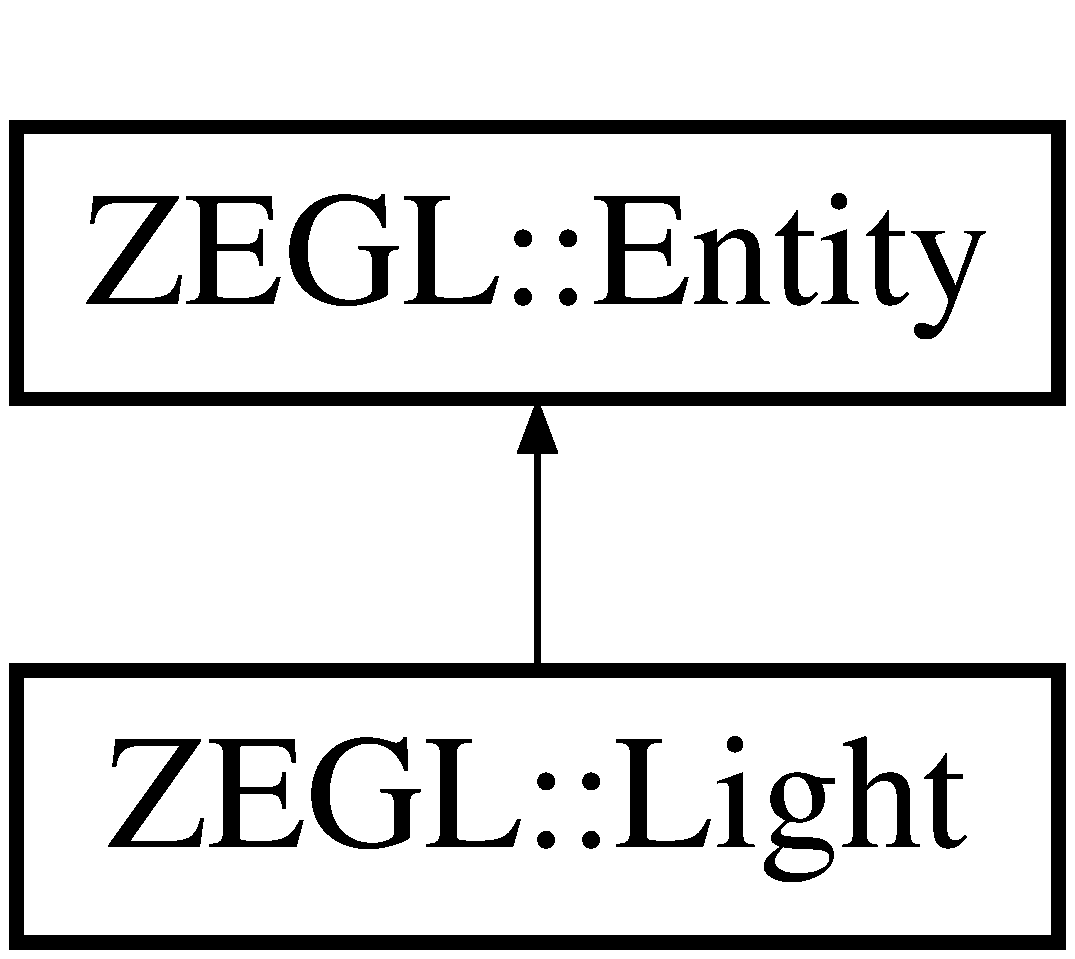
\includegraphics[height=2.000000cm]{class_z_e_g_l_1_1_light}
\end{center}
\end{figure}
\subsection*{Public Member Functions}
\begin{DoxyCompactItemize}
\item 
\hypertarget{class_z_e_g_l_1_1_light_afd825de339b3628b68ba5e6f7114bf8c}{}{\bfseries Light} (const \hyperlink{class_z_e_g_l_1_1_shader}{Shader} \&shader)\label{class_z_e_g_l_1_1_light_afd825de339b3628b68ba5e6f7114bf8c}

\item 
\hypertarget{class_z_e_g_l_1_1_light_a08a2c7c4151a9bfebe9cd55c3ccbfb90}{}{\bfseries Light} (const \hyperlink{class_z_e_g_l_1_1_shader}{Shader} \&shader, const glm\+::vec3 \&pos, const glm\+::vec4 \&light\+Col, const glm\+::vec4 \&ambient\+Col, const glm\+::vec3 \&falloff)\label{class_z_e_g_l_1_1_light_a08a2c7c4151a9bfebe9cd55c3ccbfb90}

\item 
\hypertarget{class_z_e_g_l_1_1_light_a03baeda2201dc186e7cbd244b75112f3}{}const glm\+::vec4 \& {\bfseries Get\+Light\+Color} () const \label{class_z_e_g_l_1_1_light_a03baeda2201dc186e7cbd244b75112f3}

\item 
\hypertarget{class_z_e_g_l_1_1_light_a1f30c12e1eae0c76139bd656ec7a9b54}{}const float {\bfseries Get\+Light\+Intensity} () const \label{class_z_e_g_l_1_1_light_a1f30c12e1eae0c76139bd656ec7a9b54}

\item 
\hypertarget{class_z_e_g_l_1_1_light_a05177b39933c5b4f337b7559f4411697}{}const glm\+::vec4 \& {\bfseries Get\+Ambient\+Color} () const \label{class_z_e_g_l_1_1_light_a05177b39933c5b4f337b7559f4411697}

\item 
\hypertarget{class_z_e_g_l_1_1_light_a8c2c35f9689b6775f167602b7f15d10b}{}const float {\bfseries Get\+Ambient\+Intensity} () const \label{class_z_e_g_l_1_1_light_a8c2c35f9689b6775f167602b7f15d10b}

\item 
\hypertarget{class_z_e_g_l_1_1_light_a7372ec650910810a8048f05834f51ad4}{}const glm\+::vec3 \& {\bfseries Get\+Falloff} () const \label{class_z_e_g_l_1_1_light_a7372ec650910810a8048f05834f51ad4}

\item 
\hypertarget{class_z_e_g_l_1_1_light_a1cc86994bbac07d8ddfea58269414f82}{}const \hyperlink{class_z_e_g_l_1_1_shader}{Shader} \& {\bfseries Get\+Shader} () const \label{class_z_e_g_l_1_1_light_a1cc86994bbac07d8ddfea58269414f82}

\item 
\hypertarget{class_z_e_g_l_1_1_light_a6cd065d6ac3626619d604f1cc036b399}{}void {\bfseries Set\+Light\+Color} (const glm\+::vec4 \&light\+Col)\label{class_z_e_g_l_1_1_light_a6cd065d6ac3626619d604f1cc036b399}

\item 
\hypertarget{class_z_e_g_l_1_1_light_ace2c713bef08c46068528fc5d5e42f73}{}void {\bfseries Set\+Light\+Intensity} (float light\+Intensity)\label{class_z_e_g_l_1_1_light_ace2c713bef08c46068528fc5d5e42f73}

\item 
\hypertarget{class_z_e_g_l_1_1_light_aa254cfda106426ae7e9ced71d2e853bb}{}void {\bfseries Set\+Ambient\+Color} (const glm\+::vec4 \&ambient\+Col)\label{class_z_e_g_l_1_1_light_aa254cfda106426ae7e9ced71d2e853bb}

\item 
\hypertarget{class_z_e_g_l_1_1_light_a3dc02ff4e88b483a1329072b573c90a2}{}void {\bfseries Set\+Ambient\+Intensity} (float ambient\+Intensity)\label{class_z_e_g_l_1_1_light_a3dc02ff4e88b483a1329072b573c90a2}

\item 
\hypertarget{class_z_e_g_l_1_1_light_aa60721397b726b95732cf99068b017fc}{}void {\bfseries Set\+Falloff} (const glm\+::vec3 \&falloff)\label{class_z_e_g_l_1_1_light_aa60721397b726b95732cf99068b017fc}

\item 
\hypertarget{class_z_e_g_l_1_1_light_abf084fc44a8df822ac07dba7a9b8891e}{}void $\ast$ {\bfseries operator new} (size\+\_\+t i)\label{class_z_e_g_l_1_1_light_abf084fc44a8df822ac07dba7a9b8891e}

\item 
\hypertarget{class_z_e_g_l_1_1_light_a12d5bb4765b77d6bd9bbc0d9986bce8d}{}void {\bfseries operator delete} (void $\ast$p)\label{class_z_e_g_l_1_1_light_a12d5bb4765b77d6bd9bbc0d9986bce8d}

\end{DoxyCompactItemize}
\subsection*{Additional Inherited Members}


The documentation for this class was generated from the following file\+:\begin{DoxyCompactItemize}
\item 
include/light.\+h\end{DoxyCompactItemize}

\hypertarget{class_util_1_1_my_singleton}{}\section{Util\+:\+:My\+Singleton$<$ T $>$ Class Template Reference}
\label{class_util_1_1_my_singleton}\index{Util\+::\+My\+Singleton$<$ T $>$@{Util\+::\+My\+Singleton$<$ T $>$}}
\subsection*{Static Public Member Functions}
\begin{DoxyCompactItemize}
\item 
\hypertarget{class_util_1_1_my_singleton_a7786ec28b1e4608316a2564e0f4d72e3}{}static T $\ast$ {\bfseries Get\+Instance} ()\label{class_util_1_1_my_singleton_a7786ec28b1e4608316a2564e0f4d72e3}

\end{DoxyCompactItemize}


The documentation for this class was generated from the following file\+:\begin{DoxyCompactItemize}
\item 
include/util.\+h\end{DoxyCompactItemize}

\hypertarget{class_z_e_g_l_1_1_reference_counter}{}\section{Z\+E\+G\+L\+:\+:Reference\+Counter Class Reference}
\label{class_z_e_g_l_1_1_reference_counter}\index{Z\+E\+G\+L\+::\+Reference\+Counter@{Z\+E\+G\+L\+::\+Reference\+Counter}}
Inheritance diagram for Z\+E\+G\+L\+:\+:Reference\+Counter\+:\begin{figure}[H]
\begin{center}
\leavevmode
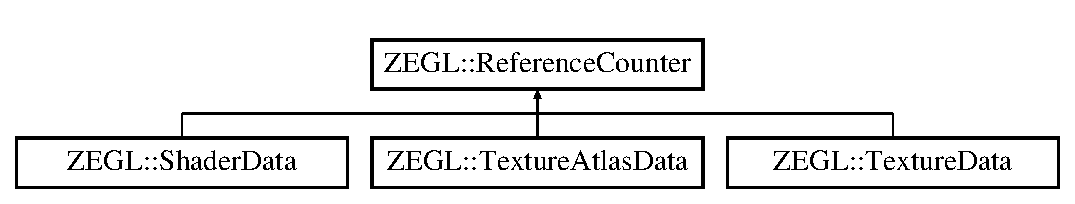
\includegraphics[height=2.000000cm]{class_z_e_g_l_1_1_reference_counter}
\end{center}
\end{figure}
\subsection*{Public Member Functions}
\begin{DoxyCompactItemize}
\item 
\hypertarget{class_z_e_g_l_1_1_reference_counter_ad417d34164157e8478947a94cd118e29}{}void {\bfseries Add\+Reference} ()\label{class_z_e_g_l_1_1_reference_counter_ad417d34164157e8478947a94cd118e29}

\item 
\hypertarget{class_z_e_g_l_1_1_reference_counter_a3118c4d9747b185355b81c033b2fd099}{}bool {\bfseries Remove\+Reference} ()\label{class_z_e_g_l_1_1_reference_counter_a3118c4d9747b185355b81c033b2fd099}

\item 
\hypertarget{class_z_e_g_l_1_1_reference_counter_a85b5de15d7d2549c17ab2c3f4b29ab01}{}int {\bfseries Get\+Reference\+Count} ()\label{class_z_e_g_l_1_1_reference_counter_a85b5de15d7d2549c17ab2c3f4b29ab01}

\end{DoxyCompactItemize}


The documentation for this class was generated from the following file\+:\begin{DoxyCompactItemize}
\item 
include/referencecounter.\+h\end{DoxyCompactItemize}

\hypertarget{class_z_e_g_l_1_1_render_entity}{}\section{Z\+E\+G\+L\+:\+:Render\+Entity Class Reference}
\label{class_z_e_g_l_1_1_render_entity}\index{Z\+E\+G\+L\+::\+Render\+Entity@{Z\+E\+G\+L\+::\+Render\+Entity}}
Inheritance diagram for Z\+E\+G\+L\+:\+:Render\+Entity\+:\begin{figure}[H]
\begin{center}
\leavevmode
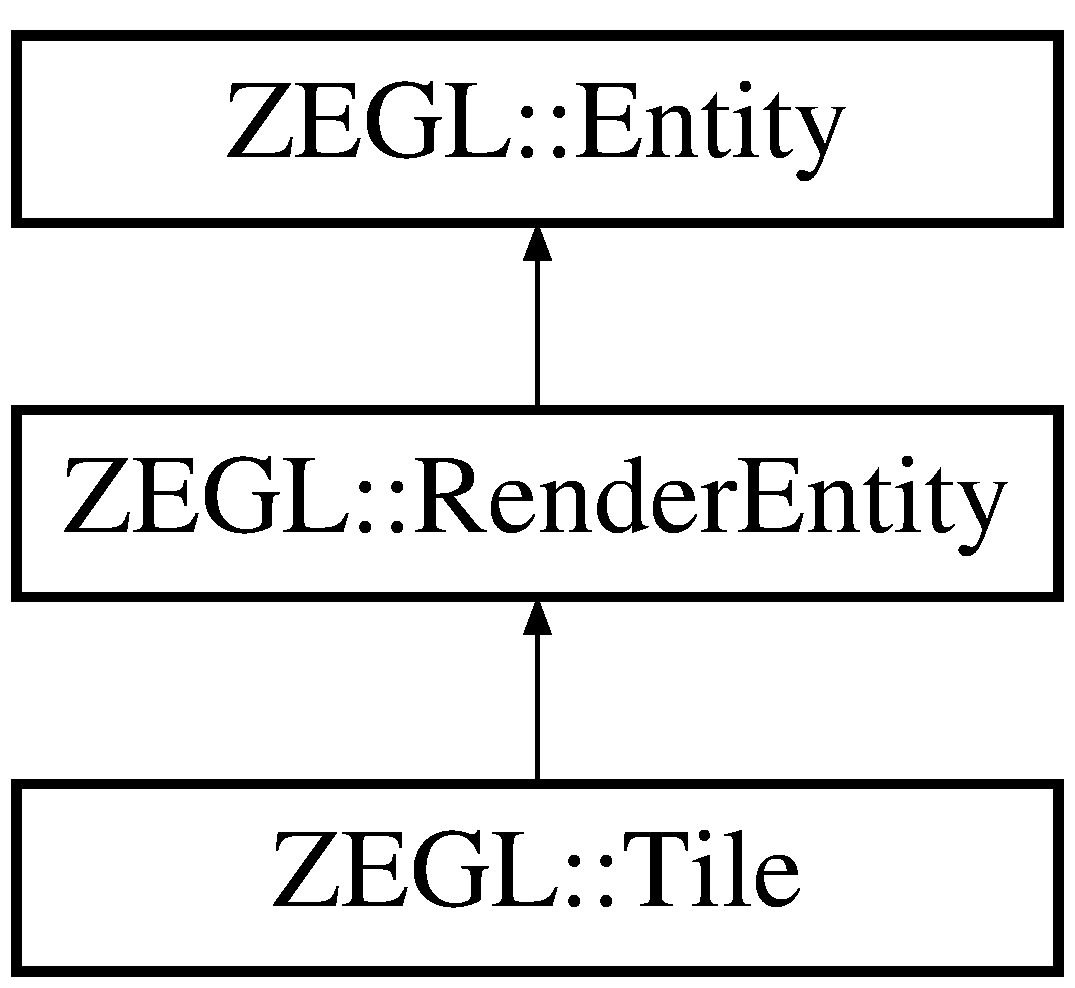
\includegraphics[height=3.000000cm]{class_z_e_g_l_1_1_render_entity}
\end{center}
\end{figure}
\subsection*{Public Member Functions}
\begin{DoxyCompactItemize}
\item 
\hypertarget{class_z_e_g_l_1_1_render_entity_a62ea0621b42dae2ec78cd39932f55c09}{}{\bfseries Render\+Entity} (const \hyperlink{class_z_e_g_l_1_1_texture}{Texture} \&texture, const \hyperlink{class_z_e_g_l_1_1_texture}{Texture} \&normal\+Map, const \hyperlink{class_z_e_g_l_1_1_texture_atlas}{Texture\+Atlas} \&texture\+Atlas, const glm\+::vec3 \&pos=glm\+::vec3(0.\+0f), float rot=0.\+0f, float scale=1.\+0f)\label{class_z_e_g_l_1_1_render_entity_a62ea0621b42dae2ec78cd39932f55c09}

\item 
\hypertarget{class_z_e_g_l_1_1_render_entity_a7421ea079ee38c841dc5dcc52f14be72}{}{\bfseries Render\+Entity} (const \hyperlink{class_z_e_g_l_1_1_texture}{Texture} \&texture, const \hyperlink{class_z_e_g_l_1_1_texture}{Texture} \&normal\+Map, const glm\+::vec2 texture\+Coords\mbox{[}4\mbox{]}, const glm\+::vec3 \&pos=glm\+::vec3(0.\+0f), float rot=0.\+0f, float scale=1.\+0f)\label{class_z_e_g_l_1_1_render_entity_a7421ea079ee38c841dc5dcc52f14be72}

\item 
\hypertarget{class_z_e_g_l_1_1_render_entity_a2c94d84990c49135e3decc2b7a24d6ea}{}{\bfseries Render\+Entity} (const \hyperlink{class_z_e_g_l_1_1_render_entity}{Render\+Entity} \&render\+Entity)\label{class_z_e_g_l_1_1_render_entity_a2c94d84990c49135e3decc2b7a24d6ea}

\item 
\hypertarget{class_z_e_g_l_1_1_render_entity_a6fb2edd900e3d39a57b3b2e2b151e203}{}void {\bfseries operator=} (\hyperlink{class_z_e_g_l_1_1_render_entity}{Render\+Entity} render\+Entity)\label{class_z_e_g_l_1_1_render_entity_a6fb2edd900e3d39a57b3b2e2b151e203}

\item 
\hypertarget{class_z_e_g_l_1_1_render_entity_a02454ceb0eb45e5761ed75f2d2095635}{}bool {\bfseries Calc\+Texture\+Coords} (const std\+::string region\+Name)\label{class_z_e_g_l_1_1_render_entity_a02454ceb0eb45e5761ed75f2d2095635}

\item 
\hypertarget{class_z_e_g_l_1_1_render_entity_a7c95293c7f110c9e67e0a0880f3120cb}{}const \hyperlink{class_z_e_g_l_1_1_texture}{Texture} \& {\bfseries Get\+Texture} () const \label{class_z_e_g_l_1_1_render_entity_a7c95293c7f110c9e67e0a0880f3120cb}

\item 
\hypertarget{class_z_e_g_l_1_1_render_entity_a547aec5a4700b863e1a5e16ead4e7119}{}const \hyperlink{class_z_e_g_l_1_1_texture}{Texture} \& {\bfseries Get\+Normal\+Map} () const \label{class_z_e_g_l_1_1_render_entity_a547aec5a4700b863e1a5e16ead4e7119}

\end{DoxyCompactItemize}
\subsection*{Protected Attributes}
\begin{DoxyCompactItemize}
\item 
\hypertarget{class_z_e_g_l_1_1_render_entity_a52be90c41c3efc4da8ac08850e86590e}{}\hyperlink{class_z_e_g_l_1_1_texture_atlas}{Texture\+Atlas} {\bfseries m\+\_\+texture\+Atlas}\label{class_z_e_g_l_1_1_render_entity_a52be90c41c3efc4da8ac08850e86590e}

\item 
\hypertarget{class_z_e_g_l_1_1_render_entity_aa6b8685142c9f25a497968613c992ce9}{}\hyperlink{class_z_e_g_l_1_1_texture}{Texture} {\bfseries m\+\_\+texture}\label{class_z_e_g_l_1_1_render_entity_aa6b8685142c9f25a497968613c992ce9}

\item 
\hypertarget{class_z_e_g_l_1_1_render_entity_aa3e87b641a10302e2f17cf18069c8c63}{}\hyperlink{class_z_e_g_l_1_1_texture}{Texture} {\bfseries m\+\_\+normal\+Map}\label{class_z_e_g_l_1_1_render_entity_aa3e87b641a10302e2f17cf18069c8c63}

\item 
\hypertarget{class_z_e_g_l_1_1_render_entity_ab8efc85bf2a85f8762ea51c0f749238f}{}bool {\bfseries m\+\_\+has\+Texture\+Atlas}\label{class_z_e_g_l_1_1_render_entity_ab8efc85bf2a85f8762ea51c0f749238f}

\end{DoxyCompactItemize}


The documentation for this class was generated from the following files\+:\begin{DoxyCompactItemize}
\item 
include/entity.\+h\item 
src/entity.\+cpp\end{DoxyCompactItemize}

\hypertarget{class_z_e_g_l_1_1_shader}{}\section{Z\+E\+G\+L\+:\+:Shader Class Reference}
\label{class_z_e_g_l_1_1_shader}\index{Z\+E\+G\+L\+::\+Shader@{Z\+E\+G\+L\+::\+Shader}}
\subsection*{Public Member Functions}
\begin{DoxyCompactItemize}
\item 
\hypertarget{class_z_e_g_l_1_1_shader_af8077122b1822f29e9fb7e199305fa52}{}{\bfseries Shader} (const std\+::string \&file\+Name=\char`\"{}basic\+\_\+shader\char`\"{})\label{class_z_e_g_l_1_1_shader_af8077122b1822f29e9fb7e199305fa52}

\item 
\hypertarget{class_z_e_g_l_1_1_shader_adab8e450ec1f4509c1bdf147e47a871c}{}{\bfseries Shader} (const \hyperlink{class_z_e_g_l_1_1_shader}{Shader} \&other)\label{class_z_e_g_l_1_1_shader_adab8e450ec1f4509c1bdf147e47a871c}

\item 
\hypertarget{class_z_e_g_l_1_1_shader_a622af0755141fc6286d3f0a50c294239}{}void {\bfseries Load} (const std\+::string \&file\+Name)\label{class_z_e_g_l_1_1_shader_a622af0755141fc6286d3f0a50c294239}

\item 
\hypertarget{class_z_e_g_l_1_1_shader_a80b52feb71b870447cd0f2a20ca68400}{}void {\bfseries Bind} () const \label{class_z_e_g_l_1_1_shader_a80b52feb71b870447cd0f2a20ca68400}

\item 
\hypertarget{class_z_e_g_l_1_1_shader_a437266d05c0aa8d125ec92e50dfe4d66}{}void {\bfseries Un\+Bind} () const \label{class_z_e_g_l_1_1_shader_a437266d05c0aa8d125ec92e50dfe4d66}

\item 
\hypertarget{class_z_e_g_l_1_1_shader_a1215713a36b12d48c1c94b56c889c269}{}void {\bfseries Set\+Uniformi} (const std\+::string \&uniform\+Name, int value) const \label{class_z_e_g_l_1_1_shader_a1215713a36b12d48c1c94b56c889c269}

\item 
\hypertarget{class_z_e_g_l_1_1_shader_aad923978e650300bfe1f82e6ec132fc3}{}void {\bfseries Set\+Uniformf} (const std\+::string \&uniform\+Name, float value) const \label{class_z_e_g_l_1_1_shader_aad923978e650300bfe1f82e6ec132fc3}

\item 
\hypertarget{class_z_e_g_l_1_1_shader_aadf0e03f829b7bbe67a0884023e9a69c}{}void {\bfseries Set\+Uniform\+Vector2f} (const std\+::string \&uniform\+Name, const glm\+::vec2 \&value) const \label{class_z_e_g_l_1_1_shader_aadf0e03f829b7bbe67a0884023e9a69c}

\item 
\hypertarget{class_z_e_g_l_1_1_shader_ac7b409fed639970c5a8f31fa852ccd23}{}void {\bfseries Set\+Uniform\+Vector3f} (const std\+::string \&uniform\+Name, const glm\+::vec3 \&value) const \label{class_z_e_g_l_1_1_shader_ac7b409fed639970c5a8f31fa852ccd23}

\item 
\hypertarget{class_z_e_g_l_1_1_shader_a7565988acbbca758622449bb1c12b344}{}void {\bfseries Set\+Uniform\+Vector4f} (const std\+::string \&uniform\+Name, const glm\+::vec4 \&value) const \label{class_z_e_g_l_1_1_shader_a7565988acbbca758622449bb1c12b344}

\item 
\hypertarget{class_z_e_g_l_1_1_shader_aee412b7edeb22a93ec4672c0d0e59f4d}{}void {\bfseries Set\+Uniform\+Matrix4f} (const std\+::string \&uniform\+Name, const glm\+::mat4 \&value) const \label{class_z_e_g_l_1_1_shader_aee412b7edeb22a93ec4672c0d0e59f4d}

\item 
\hypertarget{class_z_e_g_l_1_1_shader_a7019b356d7a9322219cb6c2336e89372}{}void {\bfseries Update\+Uniforms} (\hyperlink{class_z_e_g_l_1_1_game}{Game} $\ast$game) const \label{class_z_e_g_l_1_1_shader_a7019b356d7a9322219cb6c2336e89372}

\end{DoxyCompactItemize}


The documentation for this class was generated from the following files\+:\begin{DoxyCompactItemize}
\item 
include/shader.\+h\item 
src/shader.\+cpp\end{DoxyCompactItemize}

\hypertarget{class_z_e_g_l_1_1_shader_data}{}\section{Z\+E\+G\+L\+:\+:Shader\+Data Class Reference}
\label{class_z_e_g_l_1_1_shader_data}\index{Z\+E\+G\+L\+::\+Shader\+Data@{Z\+E\+G\+L\+::\+Shader\+Data}}
Inheritance diagram for Z\+E\+G\+L\+:\+:Shader\+Data\+:\begin{figure}[H]
\begin{center}
\leavevmode
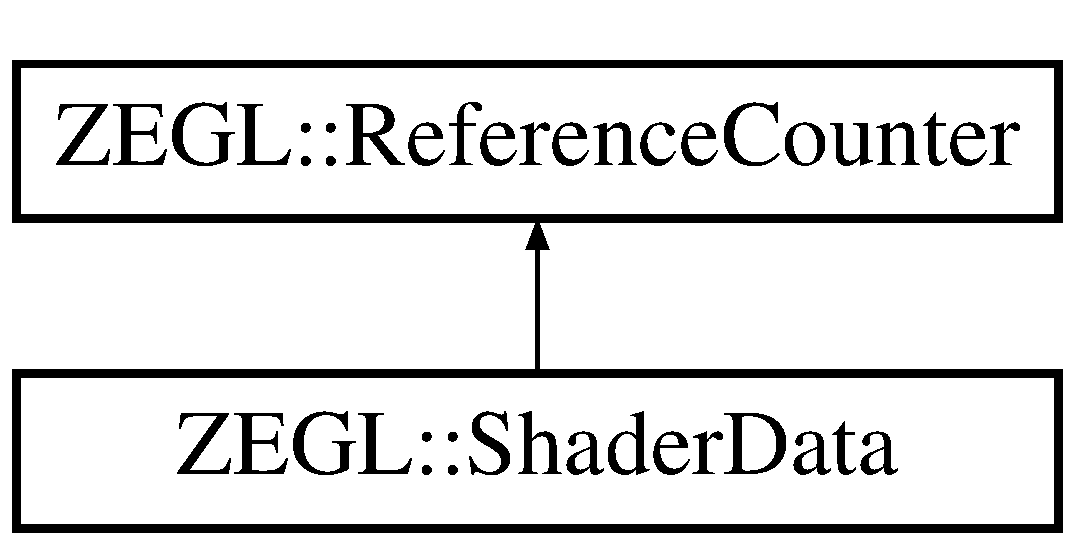
\includegraphics[height=2.000000cm]{class_z_e_g_l_1_1_shader_data}
\end{center}
\end{figure}
\subsection*{Public Member Functions}
\begin{DoxyCompactItemize}
\item 
\hypertarget{class_z_e_g_l_1_1_shader_data_a635def1584d9fbf143b1ee5941a72cf0}{}{\bfseries Shader\+Data} (const std\+::string \&file\+Name)\label{class_z_e_g_l_1_1_shader_data_a635def1584d9fbf143b1ee5941a72cf0}

\item 
\hypertarget{class_z_e_g_l_1_1_shader_data_a6c5b057d29058853bf6c4a5096f2e823}{}int {\bfseries Get\+Program} () const \label{class_z_e_g_l_1_1_shader_data_a6c5b057d29058853bf6c4a5096f2e823}

\item 
\hypertarget{class_z_e_g_l_1_1_shader_data_ac20702e6e6be0026da6b176f50c09e0c}{}const std\+::vector$<$ int $>$ \& {\bfseries Get\+Shaders} () const \label{class_z_e_g_l_1_1_shader_data_ac20702e6e6be0026da6b176f50c09e0c}

\item 
\hypertarget{class_z_e_g_l_1_1_shader_data_adc2751fc43f8f3d57051f63d5c49737d}{}const std\+::vector$<$ std\+::string $>$ \& {\bfseries Get\+Uniform\+Names} () const \label{class_z_e_g_l_1_1_shader_data_adc2751fc43f8f3d57051f63d5c49737d}

\item 
\hypertarget{class_z_e_g_l_1_1_shader_data_ac6574aa6f23427cb7e307353d1495abb}{}const std\+::vector$<$ std\+::string $>$ \& {\bfseries Get\+Uniform\+Types} () const \label{class_z_e_g_l_1_1_shader_data_ac6574aa6f23427cb7e307353d1495abb}

\item 
\hypertarget{class_z_e_g_l_1_1_shader_data_a4e4939d56d7c9c0e749c2d7f1dedfd13}{}const std\+::unordered\+\_\+map$<$ std\+::string, unsigned int $>$ \& {\bfseries Get\+Uniform\+Map} () const \label{class_z_e_g_l_1_1_shader_data_a4e4939d56d7c9c0e749c2d7f1dedfd13}

\end{DoxyCompactItemize}


The documentation for this class was generated from the following files\+:\begin{DoxyCompactItemize}
\item 
include/shader.\+h\item 
src/shader.\+cpp\end{DoxyCompactItemize}

\hypertarget{class_z_e_g_l_1_1_texture}{}\section{Z\+E\+G\+L\+:\+:Texture Class Reference}
\label{class_z_e_g_l_1_1_texture}\index{Z\+E\+G\+L\+::\+Texture@{Z\+E\+G\+L\+::\+Texture}}
\subsection*{Public Member Functions}
\begin{DoxyCompactItemize}
\item 
\hypertarget{class_z_e_g_l_1_1_texture_a211502d1cdd7812326479b1e72b09480}{}{\bfseries Texture} (const std\+::string \&file\+Name, G\+Lenum texture\+Target=G\+L\+\_\+\+T\+E\+X\+T\+U\+R\+E\+\_\+2\+D, G\+Lfloat filter=G\+L\+\_\+\+L\+I\+N\+E\+A\+R\+\_\+\+M\+I\+P\+M\+A\+P\+\_\+\+L\+I\+N\+E\+A\+R, G\+Lenum internal\+Format=G\+L\+\_\+\+R\+G\+B\+A, G\+Lenum format=G\+L\+\_\+\+R\+G\+B\+A, bool clamp=false, G\+Lenum attachment=G\+L\+\_\+\+N\+O\+N\+E)\label{class_z_e_g_l_1_1_texture_a211502d1cdd7812326479b1e72b09480}

\item 
\hypertarget{class_z_e_g_l_1_1_texture_a6a87674a108324e7b0f475850c9c9b2f}{}{\bfseries Texture} (int width=0, int height=0, unsigned char $\ast$data=nullptr, G\+Lenum texture\+Target=G\+L\+\_\+\+T\+E\+X\+T\+U\+R\+E\+\_\+2\+D, G\+Lfloat filter=G\+L\+\_\+\+L\+I\+N\+E\+A\+R\+\_\+\+M\+I\+P\+M\+A\+P\+\_\+\+L\+I\+N\+E\+A\+R, G\+Lenum internal\+Format=G\+L\+\_\+\+R\+G\+B\+A, G\+Lenum format=G\+L\+\_\+\+R\+G\+B\+A, bool clamp=false, G\+Lenum attachment=G\+L\+\_\+\+N\+O\+N\+E)\label{class_z_e_g_l_1_1_texture_a6a87674a108324e7b0f475850c9c9b2f}

\item 
\hypertarget{class_z_e_g_l_1_1_texture_a21822d3a487c6a803f706869fe46faa2}{}{\bfseries Texture} (const \hyperlink{class_z_e_g_l_1_1_texture}{Texture} \&texture)\label{class_z_e_g_l_1_1_texture_a21822d3a487c6a803f706869fe46faa2}

\item 
\hypertarget{class_z_e_g_l_1_1_texture_ac8d4a47a87bb660ecd37b7ec7a70705b}{}void {\bfseries operator=} (\hyperlink{class_z_e_g_l_1_1_texture}{Texture} texture)\label{class_z_e_g_l_1_1_texture_ac8d4a47a87bb660ecd37b7ec7a70705b}

\item 
\hypertarget{class_z_e_g_l_1_1_texture_a6f54dde94704d5f2b90c63f33c67793c}{}void {\bfseries Bind} (unsigned int unit=0) const \label{class_z_e_g_l_1_1_texture_a6f54dde94704d5f2b90c63f33c67793c}

\item 
\hypertarget{class_z_e_g_l_1_1_texture_a4e8799fb199b39f37e6f2cd33891ecfd}{}void {\bfseries Bind\+As\+Render\+Target} () const \label{class_z_e_g_l_1_1_texture_a4e8799fb199b39f37e6f2cd33891ecfd}

\item 
\hypertarget{class_z_e_g_l_1_1_texture_a057016894ae04b4a4200810e9f4c731d}{}int {\bfseries Get\+Width} () const \label{class_z_e_g_l_1_1_texture_a057016894ae04b4a4200810e9f4c731d}

\item 
\hypertarget{class_z_e_g_l_1_1_texture_a0c457e03c54b4e9ccdcd05b9d4b05c11}{}int {\bfseries Get\+Height} () const \label{class_z_e_g_l_1_1_texture_a0c457e03c54b4e9ccdcd05b9d4b05c11}

\item 
\hypertarget{class_z_e_g_l_1_1_texture_ab6b921750abf88f35c1758eeb818f3bc}{}bool {\bfseries operator==} (const \hyperlink{class_z_e_g_l_1_1_texture}{Texture} \&texture) const \label{class_z_e_g_l_1_1_texture_ab6b921750abf88f35c1758eeb818f3bc}

\item 
\hypertarget{class_z_e_g_l_1_1_texture_a1fd02861e3eba8d3b4b0aec564ea8e6c}{}bool {\bfseries operator!=} (const \hyperlink{class_z_e_g_l_1_1_texture}{Texture} \&texture) const \label{class_z_e_g_l_1_1_texture_a1fd02861e3eba8d3b4b0aec564ea8e6c}

\end{DoxyCompactItemize}


The documentation for this class was generated from the following files\+:\begin{DoxyCompactItemize}
\item 
include/texture.\+h\item 
src/texture.\+cpp\end{DoxyCompactItemize}

\hypertarget{class_z_e_g_l_1_1_texture_atlas}{}\section{Z\+E\+G\+L\+:\+:Texture\+Atlas Class Reference}
\label{class_z_e_g_l_1_1_texture_atlas}\index{Z\+E\+G\+L\+::\+Texture\+Atlas@{Z\+E\+G\+L\+::\+Texture\+Atlas}}
\subsection*{Public Member Functions}
\begin{DoxyCompactItemize}
\item 
\hypertarget{class_z_e_g_l_1_1_texture_atlas_ab33f5bce5ffa49c2d21f83603deed8df}{}{\bfseries Texture\+Atlas} (const std\+::string \&file\+Name=\char`\"{}default\+\_\+atlas.\+xml\char`\"{})\label{class_z_e_g_l_1_1_texture_atlas_ab33f5bce5ffa49c2d21f83603deed8df}

\item 
\hypertarget{class_z_e_g_l_1_1_texture_atlas_a578816352b07a4d79b21ca165c1ebe20}{}{\bfseries Texture\+Atlas} (\hyperlink{class_z_e_g_l_1_1_texture_atlas}{Texture\+Atlas} const \&)\label{class_z_e_g_l_1_1_texture_atlas_a578816352b07a4d79b21ca165c1ebe20}

\item 
\hypertarget{class_z_e_g_l_1_1_texture_atlas_a0113a9c98b3ce3aad33aa9861ad3f950}{}\hyperlink{struct_z_e_g_l_1_1_texture_region}{Texture\+Region} {\bfseries Get\+Region} (const std\+::string \&region\+Name) const \label{class_z_e_g_l_1_1_texture_atlas_a0113a9c98b3ce3aad33aa9861ad3f950}

\end{DoxyCompactItemize}


The documentation for this class was generated from the following files\+:\begin{DoxyCompactItemize}
\item 
include/textureatlas.\+h\item 
src/textureatlas.\+cpp\end{DoxyCompactItemize}

\hypertarget{class_z_e_g_l_1_1_texture_atlas_data}{}\section{Z\+E\+G\+L\+:\+:Texture\+Atlas\+Data Class Reference}
\label{class_z_e_g_l_1_1_texture_atlas_data}\index{Z\+E\+G\+L\+::\+Texture\+Atlas\+Data@{Z\+E\+G\+L\+::\+Texture\+Atlas\+Data}}
Inheritance diagram for Z\+E\+G\+L\+:\+:Texture\+Atlas\+Data\+:\begin{figure}[H]
\begin{center}
\leavevmode
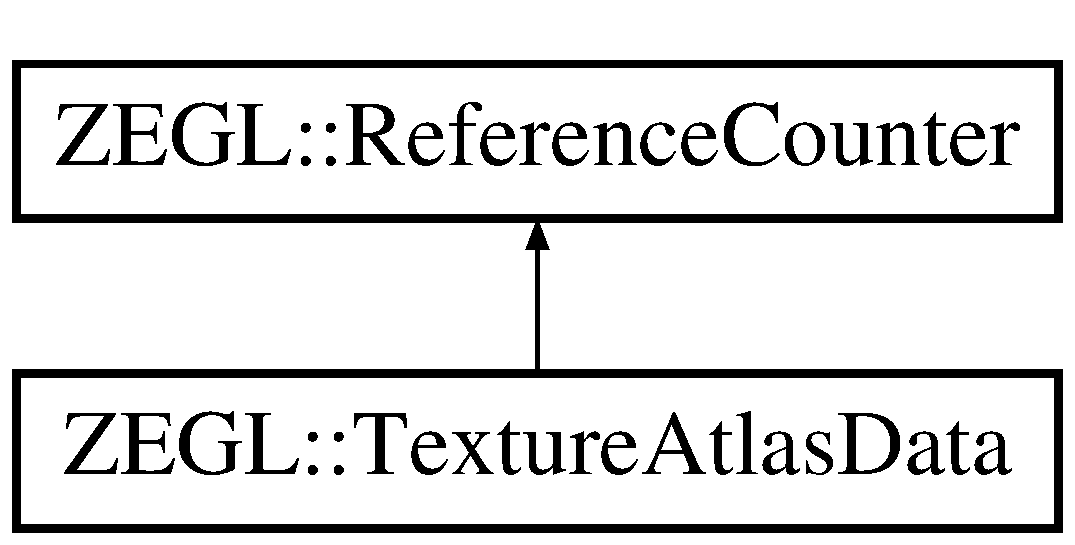
\includegraphics[height=2.000000cm]{class_z_e_g_l_1_1_texture_atlas_data}
\end{center}
\end{figure}
\subsection*{Public Member Functions}
\begin{DoxyCompactItemize}
\item 
\hypertarget{class_z_e_g_l_1_1_texture_atlas_data_a9e06ec8a09a9e8d690053b68793afc81}{}{\bfseries Texture\+Atlas\+Data} (const std\+::string \&file\+Name)\label{class_z_e_g_l_1_1_texture_atlas_data_a9e06ec8a09a9e8d690053b68793afc81}

\item 
\hypertarget{class_z_e_g_l_1_1_texture_atlas_data_a348f45893ce3dccaaa44997c5f89d8d7}{}const std\+::unordered\+\_\+map$<$ std\+::string, \hyperlink{struct_z_e_g_l_1_1_texture_region}{Texture\+Region} $>$ \& {\bfseries Get\+Regions} () const \label{class_z_e_g_l_1_1_texture_atlas_data_a348f45893ce3dccaaa44997c5f89d8d7}

\end{DoxyCompactItemize}


The documentation for this class was generated from the following files\+:\begin{DoxyCompactItemize}
\item 
include/textureatlas.\+h\item 
src/textureatlas.\+cpp\end{DoxyCompactItemize}

\hypertarget{class_z_e_g_l_1_1_texture_data}{}\section{Z\+E\+G\+L\+:\+:Texture\+Data Class Reference}
\label{class_z_e_g_l_1_1_texture_data}\index{Z\+E\+G\+L\+::\+Texture\+Data@{Z\+E\+G\+L\+::\+Texture\+Data}}
Inheritance diagram for Z\+E\+G\+L\+:\+:Texture\+Data\+:\begin{figure}[H]
\begin{center}
\leavevmode
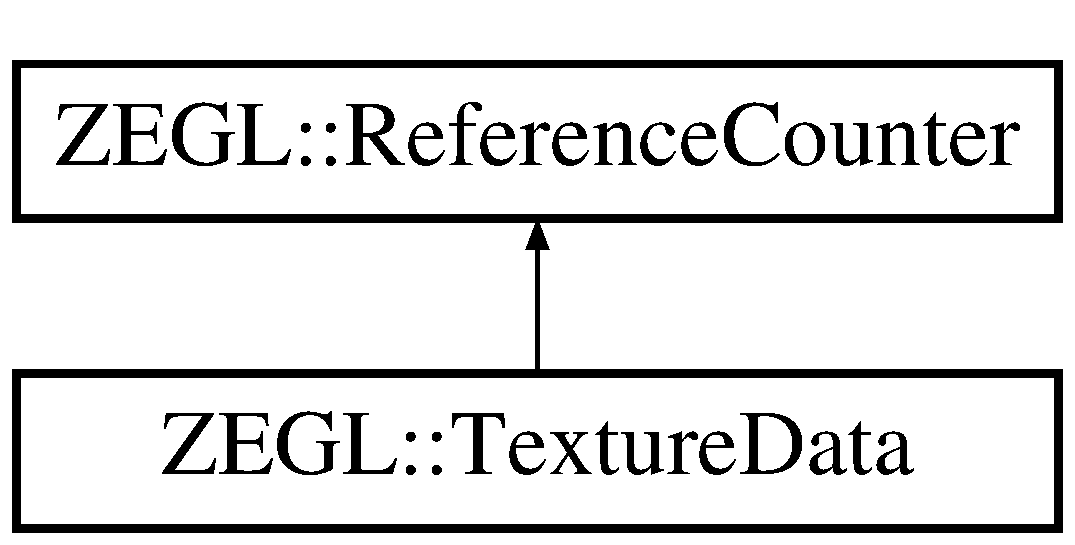
\includegraphics[height=2.000000cm]{class_z_e_g_l_1_1_texture_data}
\end{center}
\end{figure}
\subsection*{Public Member Functions}
\begin{DoxyCompactItemize}
\item 
\hypertarget{class_z_e_g_l_1_1_texture_data_ab46f64eb53b9f4dd34c936620c0f6ddb}{}{\bfseries Texture\+Data} (G\+Lenum texture\+Target, int width, int height, int num\+Textures, unsigned char $\ast$$\ast$data, G\+Lfloat $\ast$filters, G\+Lenum $\ast$internal\+Format, G\+Lenum $\ast$format, bool clamp, G\+Lenum $\ast$attachments)\label{class_z_e_g_l_1_1_texture_data_ab46f64eb53b9f4dd34c936620c0f6ddb}

\item 
\hypertarget{class_z_e_g_l_1_1_texture_data_aded7e6ed8e417bf39f815a671a0d84f8}{}void {\bfseries Bind} (int texture\+Num) const \label{class_z_e_g_l_1_1_texture_data_aded7e6ed8e417bf39f815a671a0d84f8}

\item 
\hypertarget{class_z_e_g_l_1_1_texture_data_a8d9a3f90f7656e1740e7ed3462f6458f}{}void {\bfseries Bind\+As\+Render\+Target} () const \label{class_z_e_g_l_1_1_texture_data_a8d9a3f90f7656e1740e7ed3462f6458f}

\item 
\hypertarget{class_z_e_g_l_1_1_texture_data_a22d1c6acdece9d58b0d71ebcc45cea44}{}int {\bfseries Get\+Width} () const \label{class_z_e_g_l_1_1_texture_data_a22d1c6acdece9d58b0d71ebcc45cea44}

\item 
\hypertarget{class_z_e_g_l_1_1_texture_data_ae32bf32bc742289a44460760ee23c269}{}int {\bfseries Get\+Height} () const \label{class_z_e_g_l_1_1_texture_data_ae32bf32bc742289a44460760ee23c269}

\end{DoxyCompactItemize}


The documentation for this class was generated from the following files\+:\begin{DoxyCompactItemize}
\item 
include/texture.\+h\item 
src/texture.\+cpp\end{DoxyCompactItemize}

\hypertarget{struct_z_e_g_l_1_1_texture_region}{}\section{Z\+E\+G\+L\+:\+:Texture\+Region Struct Reference}
\label{struct_z_e_g_l_1_1_texture_region}\index{Z\+E\+G\+L\+::\+Texture\+Region@{Z\+E\+G\+L\+::\+Texture\+Region}}
\subsection*{Public Attributes}
\begin{DoxyCompactItemize}
\item 
\hypertarget{struct_z_e_g_l_1_1_texture_region_a776089615c6024fe3caf49015652d7b0}{}float {\bfseries x}\label{struct_z_e_g_l_1_1_texture_region_a776089615c6024fe3caf49015652d7b0}

\item 
\hypertarget{struct_z_e_g_l_1_1_texture_region_a18d02a5caa744b525aae3c43a2a67e84}{}float {\bfseries y}\label{struct_z_e_g_l_1_1_texture_region_a18d02a5caa744b525aae3c43a2a67e84}

\item 
\hypertarget{struct_z_e_g_l_1_1_texture_region_a7a7b2967b9fa0480e0ed88e0b212cf0b}{}float {\bfseries w}\label{struct_z_e_g_l_1_1_texture_region_a7a7b2967b9fa0480e0ed88e0b212cf0b}

\item 
\hypertarget{struct_z_e_g_l_1_1_texture_region_a264c0547f1c253a4da16d05eed235920}{}float {\bfseries h}\label{struct_z_e_g_l_1_1_texture_region_a264c0547f1c253a4da16d05eed235920}

\end{DoxyCompactItemize}


The documentation for this struct was generated from the following file\+:\begin{DoxyCompactItemize}
\item 
include/textureatlas.\+h\end{DoxyCompactItemize}

\hypertarget{class_z_e_g_l_1_1_tile}{}\section{Z\+E\+G\+L\+:\+:Tile Class Reference}
\label{class_z_e_g_l_1_1_tile}\index{Z\+E\+G\+L\+::\+Tile@{Z\+E\+G\+L\+::\+Tile}}
Inheritance diagram for Z\+E\+G\+L\+:\+:Tile\+:\begin{figure}[H]
\begin{center}
\leavevmode
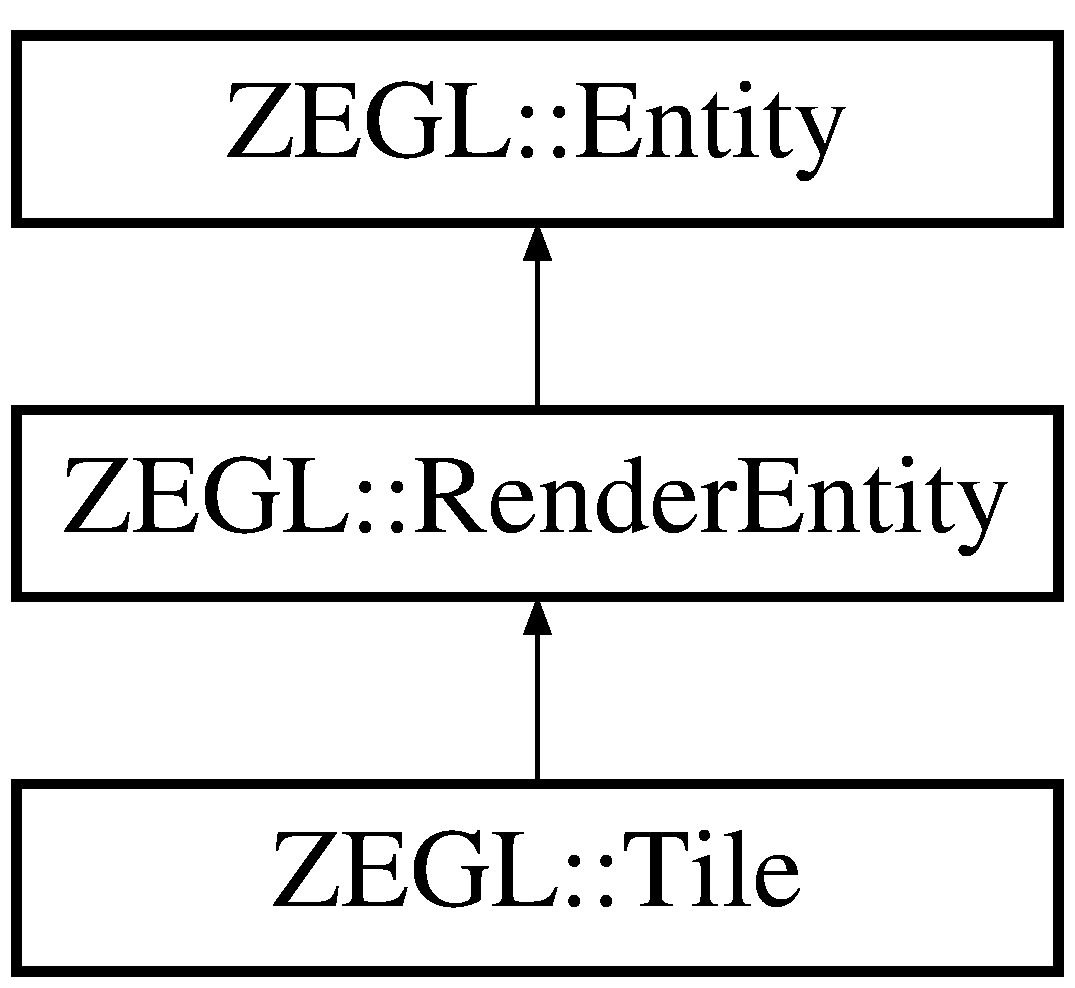
\includegraphics[height=3.000000cm]{class_z_e_g_l_1_1_tile}
\end{center}
\end{figure}
\subsection*{Public Member Functions}
\begin{DoxyCompactItemize}
\item 
\hypertarget{class_z_e_g_l_1_1_tile_a76ae8e0d534409de3973c6d3b4316060}{}{\bfseries Tile} (const \hyperlink{class_z_e_g_l_1_1_texture}{Texture} \&texture, const \hyperlink{class_z_e_g_l_1_1_texture}{Texture} \&normal\+Map, const \hyperlink{class_z_e_g_l_1_1_texture_atlas}{Texture\+Atlas} \&texture\+Atlas, const glm\+::vec3 \&pos=glm\+::vec3(0.\+0f), float rot=0.\+0f, float scale=(float) D\+E\+F\+A\+U\+L\+T\+\_\+\+T\+I\+L\+E\+\_\+\+S\+I\+Z\+E)\label{class_z_e_g_l_1_1_tile_a76ae8e0d534409de3973c6d3b4316060}

\item 
\hypertarget{class_z_e_g_l_1_1_tile_aada416574e744f9bb834e3b13d47a711}{}{\bfseries Tile} (const \hyperlink{class_z_e_g_l_1_1_texture}{Texture} \&texture, const \hyperlink{class_z_e_g_l_1_1_texture}{Texture} \&normal\+Map, const glm\+::vec2 texture\+Coords\mbox{[}4\mbox{]}, const glm\+::vec3 \&pos=glm\+::vec3(0.\+0f), float rot=0.\+0f, float scale=(float) D\+E\+F\+A\+U\+L\+T\+\_\+\+T\+I\+L\+E\+\_\+\+S\+I\+Z\+E)\label{class_z_e_g_l_1_1_tile_aada416574e744f9bb834e3b13d47a711}

\item 
\hypertarget{class_z_e_g_l_1_1_tile_afb482bccc935de5dd1cf7f6f8cdcc7c0}{}{\bfseries Tile} (const \hyperlink{class_z_e_g_l_1_1_tile}{Tile} \&tile)\label{class_z_e_g_l_1_1_tile_afb482bccc935de5dd1cf7f6f8cdcc7c0}

\end{DoxyCompactItemize}
\subsection*{Additional Inherited Members}


The documentation for this class was generated from the following files\+:\begin{DoxyCompactItemize}
\item 
include/tilemap.\+h\item 
src/tilemap.\+cpp\end{DoxyCompactItemize}

\hypertarget{struct_z_e_g_l_1_1_tile_definition}{}\section{Z\+E\+G\+L\+:\+:Tile\+Definition Struct Reference}
\label{struct_z_e_g_l_1_1_tile_definition}\index{Z\+E\+G\+L\+::\+Tile\+Definition@{Z\+E\+G\+L\+::\+Tile\+Definition}}
\subsection*{Public Attributes}
\begin{DoxyCompactItemize}
\item 
\hypertarget{struct_z_e_g_l_1_1_tile_definition_a383fb02a80f3b673f641bd2f63b5111c}{}std\+::string {\bfseries tilename}\label{struct_z_e_g_l_1_1_tile_definition_a383fb02a80f3b673f641bd2f63b5111c}

\item 
\hypertarget{struct_z_e_g_l_1_1_tile_definition_ae967508462db81a11324cc1b44865437}{}std\+::string {\bfseries texture\+Name}\label{struct_z_e_g_l_1_1_tile_definition_ae967508462db81a11324cc1b44865437}

\item 
\hypertarget{struct_z_e_g_l_1_1_tile_definition_a8e72e785cf2a4b06542bbe968f46d2be}{}std\+::string {\bfseries normal\+Map\+Name}\label{struct_z_e_g_l_1_1_tile_definition_a8e72e785cf2a4b06542bbe968f46d2be}

\item 
\hypertarget{struct_z_e_g_l_1_1_tile_definition_aa6c3b90601b4a68e83eb39eb921c9647}{}std\+::string {\bfseries texture\+Atlas\+Name}\label{struct_z_e_g_l_1_1_tile_definition_aa6c3b90601b4a68e83eb39eb921c9647}

\end{DoxyCompactItemize}


The documentation for this struct was generated from the following file\+:\begin{DoxyCompactItemize}
\item 
include/tilemap.\+h\end{DoxyCompactItemize}

\hypertarget{class_z_e_g_l_1_1_tile_map}{}\section{Z\+E\+G\+L\+:\+:Tile\+Map Class Reference}
\label{class_z_e_g_l_1_1_tile_map}\index{Z\+E\+G\+L\+::\+Tile\+Map@{Z\+E\+G\+L\+::\+Tile\+Map}}
\subsection*{Public Member Functions}
\begin{DoxyCompactItemize}
\item 
\hypertarget{class_z_e_g_l_1_1_tile_map_a40036e023361a947e946214d6b5a8c05}{}{\bfseries Tile\+Map} (const std\+::string \&file\+Name)\label{class_z_e_g_l_1_1_tile_map_a40036e023361a947e946214d6b5a8c05}

\item 
\hypertarget{class_z_e_g_l_1_1_tile_map_a8eb181de4646c39a17f9fc82267d2bfe}{}void {\bfseries Update} (float delta)\label{class_z_e_g_l_1_1_tile_map_a8eb181de4646c39a17f9fc82267d2bfe}

\item 
\hypertarget{class_z_e_g_l_1_1_tile_map_abad39ce2b672a79d6ce52145aaa7672c}{}void {\bfseries Update\+Active\+Tiles} (const \hyperlink{class_z_e_g_l_1_1_window}{Window} $\ast$window, const glm\+::vec3 \&camera\+Pos)\label{class_z_e_g_l_1_1_tile_map_abad39ce2b672a79d6ce52145aaa7672c}

\item 
\hypertarget{class_z_e_g_l_1_1_tile_map_ae52f183a2710f7dc2835fbc02ea3a81c}{}const std\+::vector$<$ \hyperlink{class_z_e_g_l_1_1_tile}{Tile} $>$ \& {\bfseries Get\+Active\+Tiles} () const \label{class_z_e_g_l_1_1_tile_map_ae52f183a2710f7dc2835fbc02ea3a81c}

\item 
\hypertarget{class_z_e_g_l_1_1_tile_map_a49f94f1a578a4a25fb15bf1dfde1ab26}{}const std\+::vector$<$ \hyperlink{struct_z_e_g_l_1_1_entity_data}{Entity\+Data} $>$ \& {\bfseries Get\+Active\+Tiles\+Data} () const \label{class_z_e_g_l_1_1_tile_map_a49f94f1a578a4a25fb15bf1dfde1ab26}

\end{DoxyCompactItemize}


The documentation for this class was generated from the following files\+:\begin{DoxyCompactItemize}
\item 
include/tilemap.\+h\item 
src/tilemap.\+cpp\end{DoxyCompactItemize}

\hypertarget{class_z_e_g_l_1_1_timer}{}\section{Z\+E\+G\+L\+:\+:Timer Class Reference}
\label{class_z_e_g_l_1_1_timer}\index{Z\+E\+G\+L\+::\+Timer@{Z\+E\+G\+L\+::\+Timer}}
\subsection*{Public Member Functions}
\begin{DoxyCompactItemize}
\item 
\hypertarget{class_z_e_g_l_1_1_timer_ab9ebe5f7765d5c0cc2644e5f575cd0b1}{}void {\bfseries Start} ()\label{class_z_e_g_l_1_1_timer_ab9ebe5f7765d5c0cc2644e5f575cd0b1}

\item 
\hypertarget{class_z_e_g_l_1_1_timer_a3a25a38b5ae28e4980cf7e0895c6f340}{}double {\bfseries Stop} ()\label{class_z_e_g_l_1_1_timer_a3a25a38b5ae28e4980cf7e0895c6f340}

\item 
\hypertarget{class_z_e_g_l_1_1_timer_a05e1d44ab7862a07008d702e32dd851e}{}void {\bfseries Restart} ()\label{class_z_e_g_l_1_1_timer_a05e1d44ab7862a07008d702e32dd851e}

\item 
\hypertarget{class_z_e_g_l_1_1_timer_af413f2b09ec51549c933d3ab5ec7437d}{}double {\bfseries Get\+Ticks} ()\label{class_z_e_g_l_1_1_timer_af413f2b09ec51549c933d3ab5ec7437d}

\end{DoxyCompactItemize}


The documentation for this class was generated from the following file\+:\begin{DoxyCompactItemize}
\item 
include/timer.\+h\end{DoxyCompactItemize}

\hypertarget{class_z_e_g_l_1_1_window}{}\section{Z\+E\+G\+L\+:\+:Window Class Reference}
\label{class_z_e_g_l_1_1_window}\index{Z\+E\+G\+L\+::\+Window@{Z\+E\+G\+L\+::\+Window}}
\subsection*{Public Member Functions}
\begin{DoxyCompactItemize}
\item 
\hypertarget{class_z_e_g_l_1_1_window_a2bf7954f0cf38a7fc4c4742e4a91a190}{}{\bfseries Window} (int width, int height, const std\+::string \&title)\label{class_z_e_g_l_1_1_window_a2bf7954f0cf38a7fc4c4742e4a91a190}

\item 
\hypertarget{class_z_e_g_l_1_1_window_ab8d28dce3166c70eb5744466460795df}{}void {\bfseries Update} ()\label{class_z_e_g_l_1_1_window_ab8d28dce3166c70eb5744466460795df}

\item 
\hypertarget{class_z_e_g_l_1_1_window_abe1b83eda6980f2b9964aab08b5310ed}{}void {\bfseries Swap\+Buffers} ()\label{class_z_e_g_l_1_1_window_abe1b83eda6980f2b9964aab08b5310ed}

\item 
\hypertarget{class_z_e_g_l_1_1_window_a7b9db9583287699589b2cd8414eb8ca3}{}void {\bfseries Bind\+As\+Render\+Target} () const \label{class_z_e_g_l_1_1_window_a7b9db9583287699589b2cd8414eb8ca3}

\item 
\hypertarget{class_z_e_g_l_1_1_window_a1dfc1788b9219491978175766665ecf3}{}bool {\bfseries Is\+Close\+Requested} () const \label{class_z_e_g_l_1_1_window_a1dfc1788b9219491978175766665ecf3}

\item 
\hypertarget{class_z_e_g_l_1_1_window_a72d51a5848206c942eef6155b58c43bd}{}int {\bfseries Get\+Width} () const \label{class_z_e_g_l_1_1_window_a72d51a5848206c942eef6155b58c43bd}

\item 
\hypertarget{class_z_e_g_l_1_1_window_ad7886b325583ea1059878e822c7f080d}{}int {\bfseries Get\+Height} () const \label{class_z_e_g_l_1_1_window_ad7886b325583ea1059878e822c7f080d}

\item 
\hypertarget{class_z_e_g_l_1_1_window_a2125db36818bd9110a28658b6e8e3d85}{}float {\bfseries Get\+Aspect} () const \label{class_z_e_g_l_1_1_window_a2125db36818bd9110a28658b6e8e3d85}

\item 
\hypertarget{class_z_e_g_l_1_1_window_a0acad71a1f0532baadda1d84a6e063ca}{}const std\+::string \& {\bfseries Get\+Title} () const \label{class_z_e_g_l_1_1_window_a0acad71a1f0532baadda1d84a6e063ca}

\item 
\hypertarget{class_z_e_g_l_1_1_window_ab38a9c7f9d73195fc84ab0b04b2bfbad}{}glm\+::vec2 {\bfseries Get\+Center} () const \label{class_z_e_g_l_1_1_window_ab38a9c7f9d73195fc84ab0b04b2bfbad}

\item 
\hypertarget{class_z_e_g_l_1_1_window_ac563daa5dc6417b74601b05aa87fd5b8}{}S\+D\+L\+\_\+\+Window $\ast$ {\bfseries Get\+S\+D\+L\+Window} ()\label{class_z_e_g_l_1_1_window_ac563daa5dc6417b74601b05aa87fd5b8}

\item 
\hypertarget{class_z_e_g_l_1_1_window_a4484df799a60648fa9f4cf732a963bf0}{}const \hyperlink{class_z_e_g_l_1_1_input}{Input} \& {\bfseries Get\+Input} () const \label{class_z_e_g_l_1_1_window_a4484df799a60648fa9f4cf732a963bf0}

\item 
\hypertarget{class_z_e_g_l_1_1_window_a5aca5526280a2f95f42c732a407a6129}{}void {\bfseries Set\+Full\+Screen} (bool value)\label{class_z_e_g_l_1_1_window_a5aca5526280a2f95f42c732a407a6129}

\end{DoxyCompactItemize}


The documentation for this class was generated from the following files\+:\begin{DoxyCompactItemize}
\item 
include/window.\+h\item 
src/window.\+cpp\end{DoxyCompactItemize}

%--- End generated contents ---

% Index
\backmatter
\newpage
\phantomsection
\clearemptydoublepage
\addcontentsline{toc}{chapter}{Index}
\printindex

\end{document}
